\documentclass[authoryearcitations]{UoYCSproject}
\usepackage[utf8]{inputenc} 
% \usepackage[parfill]{parskip}
\usepackage{pgfplots, pgfplotstable}
    \pgfplotsset{%
    	% every tick label/.append style={scale=1.5},
        compat=newest,%
        % /pgf/number format/use comma,%
        /pgf/number format/1000 sep={\,},%
        /pgf/number format/min exponent for 1000 sep=4}
\usepgfplotslibrary{statistics}


\areaset{445pt}{610pt}
\usepackage{mathtools}
\usepackage[numbers]{natbib}
\usepackage{filecontents}
\usepackage{listings}
\usepackage{graphicx}
\usepackage{scrhack}
\usepackage{hyperref}
\usepackage{amsthm}
\usepackage{cleveref}
\usepackage{wrapfig}
\usepackage{multicol}
\usepackage{float}

\usepackage{subcaption} 
\author{Miguel D. Boland}
\title{Evolutionary algorithms for indoor localisation}
\date{\today}
\supervisor{Leandro S. Indrusiak}
\MEng
\wordcount{wordcount}

% \includes{Appendices \ref{cha:usefulpackages}, \ref{cha:gotchas} and
%   \ref{cha:deptfac}}


\abstract{}


\begin{document}

\maketitle
% \tableofcontents
\listoffigures
\listoftables
\clearpage
% \renewcommand*{\lstlistlistingname}{List of Listings}
\lstlistoflistings
\begin{itemize}
	\item ICP: Iterative Closest Point algorithm
	\item NDT: Normal distribution transform
	\item EA: Evolutionary Algorithm
	\item PSM: Polar Scan matching
	\item HSM: histogram scan matching
	\item PCA: Principal Component Analysis
	\item GLASM: Genetic Lookup based Algorithm for Scan Matching
	\item h-GLASM: Hybrid Genetic Lookup Based Algorithm for Scan Matching
	\item DGA: Dynamic Genetic Algorithm
\end{itemize}


\chapter{Introduction}
\label{cha:Introduction}
Indoor localisation is the process of locating an electronic device's orientation and position within the confines of an indoor environment, for the purpose of conducting a location-dependent activity \cite{Curran2011-zs}. An autonomous robot's ability to locate itself is key to its ability to navigate and interact with its environment where accuracy or autonomy is required. 

This proves to be a non-trivial problem due to the lack of reliability of odometers on electrical models, which are liable to cumulative errors in displacement measurement stemming from limited encoding resolution or sampling rate, in addition to variations over the surface travelled, or related wheel-slippage \cite{Borenstein1996-al}. Similarly, a talk by \citet{Sachs2010-pw} demonstrates the complexities of using accelerometers and gyroscopes for indoor positions, citing the variations in sensing errors due to temperature changes, magnetic disturbances or sharp accelerations. Finally, the use of GPS signals indoors is non-trivial due to the obstruction of signals by buildings; this is still an active area of research\cite{Gowdayyanadoddi2015-hg}. As such, indoor localisation has been an active field of research in an effort to provide autonomous systems with an ability to maintain a given displacement, in addition to the ability to locate itself within a known environment. 

The academic research into this field follows three paradigms. The first two of these involves the usage of either an ad-hoc wireless infrastructure or existing wireless infrastructure, paired with mathematical models to interpret the strength or angle of arrival of wireless signals into a pose and translation. An overview of this area of research is presented by \citet{Liu2007-in}, demonstrating a range of use of wireless technologies; his findings demonstrate the lack of a commercial wireless indoor localisation solution which is both low-cost, robust and accurate to within a a few centimetres. As such, these solutions may be unfeasible in environments requiring precise localising and manoeuvring, but could be applied in situations where further refinement could be provided by a user. 

The third paradigm for an adaptable and infrastructure-free solution to indoor localisation revolve around the use of line-of-sight based solutions: these rely on various sensor technologies to map information obtained from a  $360^{\circ}$ scan to a known map of the environment. As this method relies entirely on the environment through which the robot is attempting to navigate, it should be capable of generating a more accurate and precise indoor localisation system at a reduced cost, without depending on the availability of an optional system; this could be well adapted to emergency situations, where existing electrical infrastructure is hampered yet accurate positioning is critical to the task at hand. 


Restricting the context of this dissertation to applications in autonomous robots requiring accurate positional tracking, we can state that the scope of this project is to investigate the development of infrastructure free indoor localisation systems, and in particular the development of evolutionary algorithms for indoor positioning.

The rest of this document is organised as follows: ......


\chapter{Literature Review}

\section{Problem definition}
A common problem description for 2-dimensional indoor localisation can be defined as the search for a tuple $(x, y, \theta)$ which describes the location $x, y$ of the robot with relation to an origin, and a rotation $\theta$ from a particular orientation. This would be sufficient to solve localisation for a robot travelling on a linear plane, without consideration for changes in altitude relative to the plane.

Within the domain of indoor localisation, this problem is applied to scan matching, where a partial set of data is placed within the larger set of data using a 3-tuple transformation to maximise the overlap of data. [TODO ADD EXAMPLE/MERGE WITH NEXT SUBSECTION]


\section{Use of sensor technologies}
Starting with the selection of sensor type, we have opted to assume the use of a laser range scanner, which can provide a set of data in the form of $(d, \theta)$ where d is the distance measured when pointing the sensor at an angle $\theta$ from the centreline of the robot. As the rotation and measurement of the sensor can be handled by a packaged, stand-alone hardware component, we can assume these will be performed within the manufacturer's specifications without need for additional implementation. This benefit is reflected in research by \citet{Lingemann2005-hm}, who finds benefits in the accuracy and processing speed of data obtained from laser range scanners in comparison to sonar, stereo-cameras and omnidirectional vision.

\section{Overview of data representation strategies}
Three major paradigms exist in the approaches to the data-representation involved when mapping data from a robot's sensors and environment map. These can be described as point-point matching (raw Cartesian coordinates are used \cite{Lu1997-zv}), point-feature (points are mapped to a database of features \cite{Censi2008-ik}) and feature-feature (raw data is formed into features, which are mapped to known features \cite{Reina2000-vq}. 

Point-feature and feature-feature based localisation are two paradigms of indoor localisation. These rely on the ability to identify features in the robot's environment, and relate these to known features in order to retrieve the robot's pose. As overviewed by \citet{Filliat2003-ay}, approaches include utilising corners \cite{Borghi1995-pi} \cite{Hebert1996-rc}, lines \cite{Moutarlier1990-ld} \cite{Einsele1997-dl}, cylinders and planes \cite{Leonard1990-hx}, or finally higher level features \cite{Ayache1990-ok}. These methods aim to reduce the complexity of the matching section by pre-processing the available information; this may not afford any considerable benefit as it balances this reduction in complexity with the need to identify features in the raw scan data. As such we have decided to focus this project on a point-point approach.

As such, the problem can be stated as finding an optimal alignment of a set of relative scanned coordinates to an absolute map of the environment.

These algorithms will be reviewed in the following section:
\begin{itemize}
	\item \autoref{sec:classical_approaches} reviews pre-genetic algorithms (also known as `classical` algorithms)
	\item \autoref{sec:evo_approaches} reviews algorithms which utilise only evolutionary algorithms
	\item \autoref{sec:hybrid_approaches} reviews hybrid algorithms which combine evolutionary and classical algorithms.
\end{itemize}


\section{Classical approaches to point-to-point based localisation}
\label{sec:classical_approaches}
\subsection{Overview of classical approaches}
'Classical' approaches refer to all non-genetic algorithms reviewed in this report. These algorithms aim to retrieve a robot's pose using two scans, each composed of 2d Cartesian or polar coordinates: the first of these is a reference scan of the environment, and the second is obtained from a Li-Dar scanner. These is achieved in either a local or global scope, using a variety of heuristic methods.
\begin{figure}[t]
	\centering
	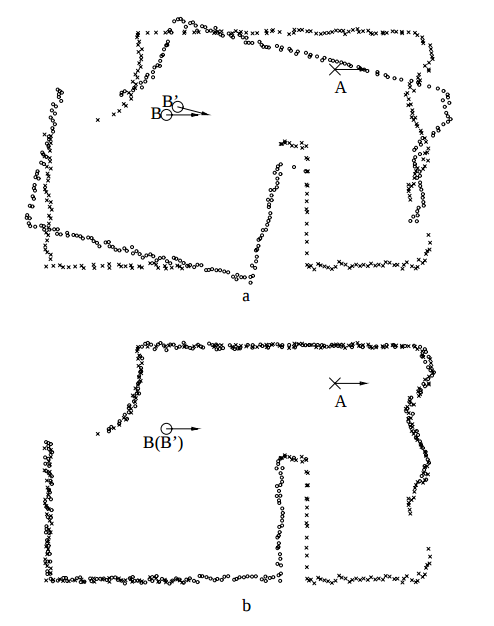
\includegraphics[width=5cm,keepaspectratio]{images/pose_estimation.png}
	\label{fig:pose_estimation}
	\caption[An example of pose registration]{An example of pose registration: the robot has moved from pose A to B, but due to odometric error believes it is in B'. Points on it's current scan B' can be transformed and rotated to overlay the points obtained from a scan at B, which would allow it the robot to obtain it's current position relative to B. Source: \citet{Lu1997-zv}.}
\end{figure}
\subsection{Iterative Closest Point and variants}
\label{subsec:ICP}
The Iterative Closest Point algorithm (ICP) is one of the first, if not the fundamental starting point for the applications of heuristic algorithms to the matching of scanned data to environment maps within the context of indoor localisation.

In this point-point data representation, the algorithm first detailed by \citet{Besl1992-pd} aims to find an optimal transformation to apply to the scan which minimises the sum of the distances measured of each scan-point to their closest point in the reference map. This can be pre-processed with the removal of points with no proximate matching point, and iteratively changing the solution tuple to minimise the error using the Newton or Lorentzian methods \cite{Munoz2005-gt}. Starting from an initial position and a scan of the environment from this position, the algorithm will converge to a local optimum alignment. 

Many improvements have been suggested (20 736 variations according to \citet{Donoso2017-wp}), which aim to improve the convergence speed \cite{Donoso2017-wp} \cite{Simon1996-dl}, removal of points from the datasets which would reduce the optimality of the solution \cite{Weik1997-px} \cite{Masuda1996-av} or the precision metric used \cite{Eggert1997-ak}. As such it continues to be a strong area of research, and can prove to be an accurate and relatively quick solution to scan matching.

However, ICP finds a local optimum from a hypothetical pose: this would inhibit the algorithm from finding a global position in a single run, and this is reflected by \citet{Censi2005-iv} who states that "any 'local' matcher can be (inefficiently) used for a global search". This could be implemented by randomising the starting pose over multiple runs, highlighting the additional complexity required to adapt this algorithm into a global search.

Nevertheless it continues to be an area of continuous research, as \citet{Minguez2006-nj} developed a version of ICP in 2006 named mbICP;  this accounts for the issue that the distance of a scanned point from the sensor will be proportional to the translation error of that point due to a rotational error. This would therefore skew the error of the hypothetical translation, potentially driving it away from a local error minima.

Similarly,TrICP \cite{Chetverikov2005-yz} implements a Trimmed Least Squares \cite{Ruppert1980-js} algorithm rather than a Least Squares, improving the robustness to noise or poor initial estimations of the pose. This functions on a subset of points, thereby preventing erroneous measurements or outliers from affecting the overall regression. The algorithm is not pareto dominant to a standard ICP, as demonstrated by \citeauthor{Chetverikov2005-yz} through the examples in \autoref{fig:trICP_misalignment}; the TrICP algorithm was unable to align the M and P scans to form the correct R scan, whereas an ICP algorithm was able to achieve this result. 


\begin{figure}[t]
	\centering
	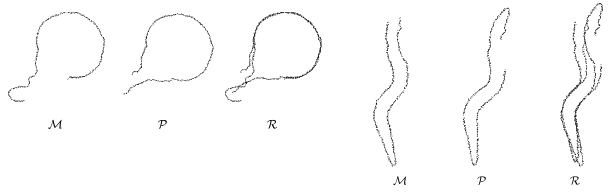
\includegraphics[width=\textwidth,keepaspectratio]{images/trICP_misalignment.png}
	\caption[TrICP mis-alignment]{TrICP mis-alignment. Source: \citet{Chetverikov2005-yz}.}
	\label{fig:trICP_misalignment}
\end{figure}

Various forms of ICP therefore out-perform each other depending on the case at hand: \citet{Donoso2017-wp} recently published a comprehensive overview of 20,736 variants of the ICP algorithm in their ability to consolidate (and therefore place relative to each other) sets of 3 sets of 100 scans at distinct locations. These variants were generated by decomposing major ICP algorithms into their components (such as their point selection criteria, neighbourhood selection, point matching, etc), and creating new algorithms using every permutation of components. He finds that the performance (precision, accuracy and computational efficiency) of ICP variants can significantly vary depending on the scan and map data, and that no single algorithm was able to adequately solve all 3 scenes in the experiment. As such, the selection of a particular variant of ICP may be significant to the effectiveness of scan matching, as we will later discuss in \ref{sec:hybrid_approaches}.


\subsection{Iterative Dual Correspondence}

The development of the IDC algorithm by \citet{Lu1997-zv} focused on the same issue in ICP for which mbICP was developed: distant points in a scan have a large matching error due to translation errors, relative to closer points. To solve this, IDC matches points in polar form. This results in a reduced computational complexity, as rather than search a 3-dimensional space, it solves an efficient one-dimensional search followed by a least squares solution. This is achieved by computing a trial value of the rotation from a global search on tangent directions from each scan, before executing a least-squares to affine the translation and rotation. This would have to be adapted for use in global localisation where the entirety of the map is not visible from a single scanning point due to range limitations, but does highlight some areas for improvement in ICP, both in terms of removing un-necessary data conversion and reducing the complexity of the algorithm. The method would also be difficult to apply to global localisation due to a lack of global search: an optimal minima would only be found if the initial error in rotation is relatively small (< 15$^o$).


\subsection{Polar Scan Matching}
\label{subsec:psm}
Polar scan matching \citet{Diosi2005-nv} utilises the same concept as IDC by adapting the ICP algorithm to use polar coordinates in an effort of minimising computational requirements. After pre-processing each scan to remove inconsistent data (due to moving objects) and segmenting the points according to a threshold criteria, the current scan is re-projected from the reference position (as demonstrated in \autoref{fig:polar_projection}, and the remaining translation and orientation is then iteratively improved. This method therefore benefits from the direct use of raw data from a laser scanner, in addition to a reduction in the dimensionality of the problem through matching the bearings of the polar data by distance. 

\begin{figure}[t]
	\centering
	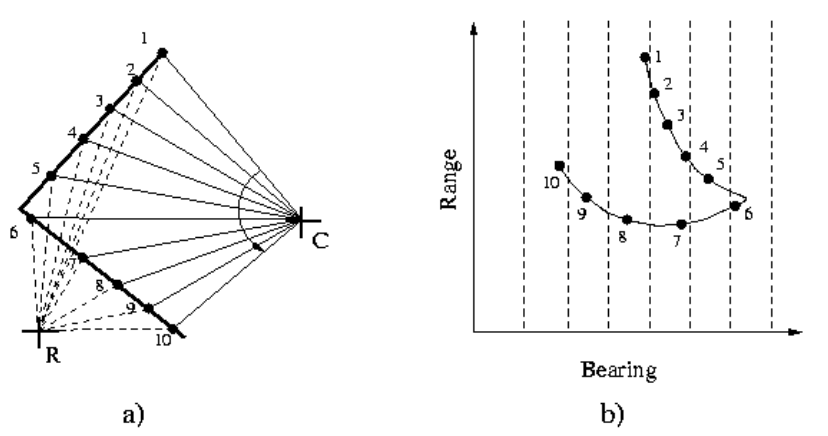
\includegraphics[width=\textwidth,keepaspectratio]{images/polar_projection.png}
	\caption[Polar Scan projection]{Polar scan projection: Points taken from location C, projected to location R. Source: \citet{Diosi2005-nv}.}
	\label{fig:polar_projection}
\end{figure}

\subsection{Principal Component Analysis}
Principal Component Analysis is a form of manifold learning which is applied to indoor localisation by constructing an eigenspace of the environment from a set of range scans taken in a 2D grid of the map. To avoid brute-forcing over every known scan of the environment, Principal Component Analysis is used to combine these, allowing subsequent scan matching to be done by measuring the relative similarity of the scan to points in the eigenmap, as each scan location will project to a point in the eigenspace. A nearest neighbour search in the eigenspace can then determine the most likely candidate pose. This nearest known pose can then be refined through odometric movement \cite{Pourraz1999-nu}, or by collective enough scans to provide a denser data-point matching sufficient to match a criteria of accuracy \citet{Pourraz1999-nu}. As such, the application of PCA to the method reduces to a classification problem, unless additional measures are taken to refine the solution. Additional computation, such as calculating the pose as an average of the coordinates of the $n$ nearest neighbours, could enhance this method to provide accurate global search, but this has not yet been investigated. 

\subsection{Normal distribution transform}
The normal distribution transform (NDT) by \citet{Biber2003-kb} is one of the first tangential research away from point set/feature matching. The set of points in a map can be converted into a piecewise probability density function over a 2D plane. This can be decomposed into a set of normal distributions, and the second scan can be matched by maximising the sum that the aligned points score on the previous density. The scan matching is hence performed in a different domain, using information preserving transformations. This is readily applicable to our case study, as a set of normal distributions of a map could be pre-computed, thereby avoiding repeated computations. As it relies on creating statistical approximations of the dataset, NDT requires a relatively dense data set for it's map representation; this has the side effect of making it extremely resilient to noisy data. This does remain a form of local search, in-line with previous attempts to produce an odometric correction algorithm rather than a generic localisation. 

\subsection{Hausdorff distance}
The usage of the Hausdorff distance was introduced by \citet{Donoso-Aguirre2008-pb}; it is defined as the maximum distance between a point in the scan and it's closest point in the map, as demonstrated in \autoref{fig:hausdorff}. As such, it signifies that every point in the scan is not any further from it's closest point in the scan than the Hausdorff distance for these sets of points. This is further improved by using the $k_{th}$ distance so as to avoid false positives due to outlying points, and instead defining the fitness function as the minimisation of the average of the first K ranked maximum Hausdorff distance. Although this could method of pose evaluation could easily be adapted into the fitness function of a genetic algorithm, the demonstrated search method would be limited to finding a local minima; without odometric data, this is unlikely to yield a global maxima. This is due to the use of an iterative gradient descent algorithm. However, the algorithm is shown to be resilient to noise and accurate when given a rough pre-alignment. Therefore, a viable adaptation of this algorithm could involve the use of coarse global search algorithm using the averaged Hausdorff as a measure of error, followed by a different algorithm to refine the roughly pre-aligned method.

\begin{figure}[t]
	\centering
	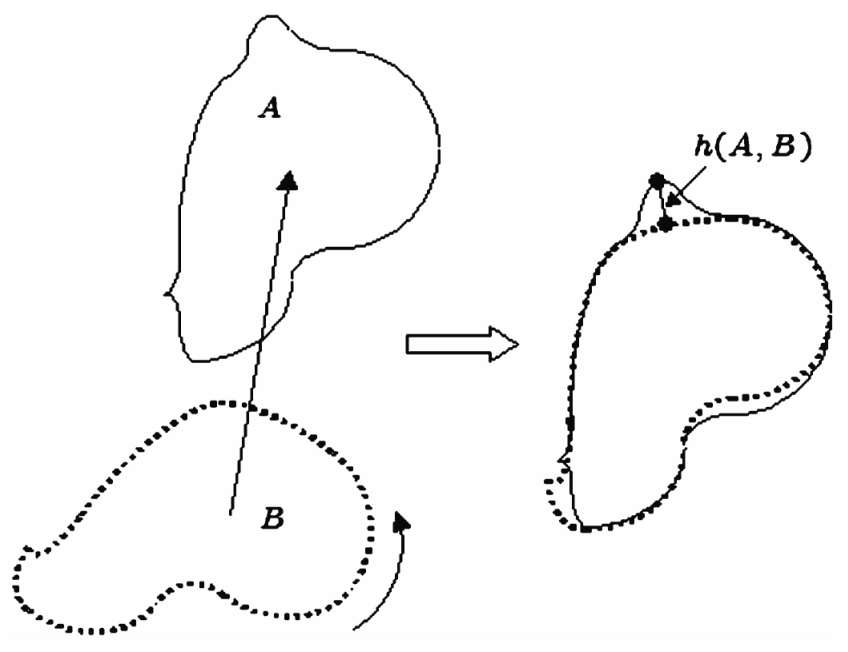
\includegraphics[width=0.5\textwidth,keepaspectratio]{images/hausdorff.png}

	\caption[Hausdorff distance]{Hausdorff distance between points in two scans.. Source: \citet{Donoso-Aguirre2008-pb}.}
	\label{fig:hausdorff}
\end{figure}

\subsection{Cross-correlation scan matching}
The Cross correlation scan matching (CCSM) algorithm functions by using the set of scan points to define a 2d form, with points in the scan forming the outline of the shape. Repeating the same process using a reference scan, we obtain two equivalent shapes which we must overlay to obtain the relative pose of our robot. This is achieved by maximising the intersected area of the two shapes, as seen in \autoref{fig:cross_correlation}, where the intersected area is darkened. The method is optimised using rasterised scanning, which also helps account for sources of noise in the sensor. \citet{Konecny2016-zv} demonstrates an improved performance compared to ICP, including a higher breadth but not global search, and a significant performance improvement. No further work is conducted to evaluate it's performance on non-solid shapes (e.g: two rooms separated by a wall and door), which may impede the algorithm's effectiveness. 

\begin{figure}[t]
	\centering
	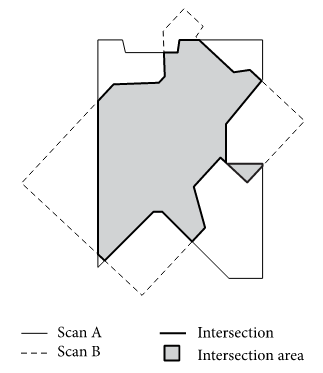
\includegraphics[width=5cm,keepaspectratio]{images/cross_correlation.png}
	\caption[Cross correlation scan matching]{Matching scans by cross correlation. Source: \citet{Konecny2016-zv}.}
	\label{fig:cross_correlation}
\end{figure}

\subsection{Hough Scan Matching}
Hough Scan Matching relies on the creation of a function which produces a spectrum from a transformed set of points (using the Hough Transform) which has the following properties; it is invariant to input translations, and is circularly shifted on the input rotation. The search is therefore performed in a different domain which was created using an information-preserving transformation. The output of the scan and map sets can then be combined using a cross-correlation operator to retrieve the relative rotation. From there, a variety of other algorithms can retrieve the most likely translation given one or more candidate rotations; the method can therefore provide a ranked output of possible pose estimations. As presented by \citet{Censi2005-iv}, hough scan matching is therefore a potent, low-complexity approach to global indoor localisation. It may be particularly adaptable to a scan-to-map application as the spectrum of the map could be pre-computed, thereby reducing the processing time for repeated pose estimations.

\subsection{Histogram scan matching}
Histogram scan matching (HSM) was first detailed by \citet{Weiss1994-ub}. It functions by creating a histogram of the range of angles between points in a scan. By building graphs of the scan and map, we can obtain two comparable histograms with some degree of phase shift matching the relative pose rotation. Aligning the two histograms using maximas and minimas would allow the retrieval of candidate rotations. The process can then be repeated using histograms of the distances between points along the x and y axis, before being matched in a similar fashion. As such, the algorithm can determine the 3-tuple pose transformation in 3 consecutive $O(n)$ operations, greatly reducing the complexity of the algorithm relative to other methods. This resulted in a global search algorithm which was tested on relatively large rotations and transitions, but lacked any comparison to other algorithms: as such it is difficult to evaluate it's relative performance. HSM can however provide a global search with a low computational cost, that is resilient to noise.

\section{Evolutionary Algorithms}
\label{sec:evo_approaches}
\subsection{Overview of genetic algorithms}
Evolutionary algorithms (EAs) are a type of meta-heuristic algorithms inspired from biological natural selection. As detailed by \citet{Whitley1994-tx}, evolutionary algorithms utilise a population of individuals, each with their own set of 'chromosomes' which would provide a solution to a given problem. These individuals are then evaluated against a stated fitness function, then selected by fitness using a competitive method which returns a 'fitter' subset of the population. This elite are then mutated to introduce a probability of improving their solution, and are crossed over with each other to share the benefits that they have inherited or mutated. This new population is then passed through the same process, and the process is repeated for a number of cycles, with each generation developing a fitter (and therefore better) solution to the given problem. 

Evolutionary algorithms therefore form an alternative to the iterative improvement strategy found in the 'classical' methods previously discussed. This divergence is notable in two ways: firstly, a large number of alternative methods used to evaluate the resultant error from a transformation/rotation tuple can be adapted into the evolutionary algorithm's fitness function, and therefore the genetic algorithm could theoretically discover equivalently optimal minima in the fitness landscape. Secondly, as the initial population can be assigned to poses distributed around the map, and the random nature of a evolutionary algorithms allow individuals to progress against a fitness gradient through mutations and cross-overs, a global optima can be found. Evolutionary algorithms therefore allow many of the previously designed algorithms to be adapted into a solution to generically locate oneself in an environment with no prior knowledge of our displacement.

The use genetic algorithms to search for data-matching was first proposed by \citet{Brunnstrom1996-vo} in \citeyear{Brunnstrom1996-vo}; this focused on the ability to find the correspondence between 2 detailed surface models. This was achieved by using a chromosome design based on a transformation, translation and rotation in 3 dimensions. As our scan matching only utilises 2-dimensional data, and temporarily ignoring the need for a transformation to handle noise, this chromosome design overcomplicates the application of scan matching in 2D indoor localisation. As such, the general chromosome design (without accounting for noise management) would simply consist of the 3-tuple previously detailed, composed of 2 transformations and a rotation.

\subsection{Parallel Evolutionary Registration of Range Data}
\citet{Robertson2002-ou} presented one of the first applications of genetic algorithms as an alternative to the ICP algorithm. Most notably, he contrasts the limitations of ICP (requiring pre-registration by hand to converge to a global minimum, tendency to converge to sub-optimal or incorrect solutions) with the benefits of a genetic algorithm; the latter does not require any form of pre-alignment, and has a significantly broader basin of convergence, allowing it to search for global solutions without any prior knowledge. This is implemented using a 3-tuple matching our problem definition, and results in significantly better global search results than a single ICP run. This therefore demonstrates the potential of genetic algorithms within the field, setting the path for following research.

\subsection{Genetic Algorithm Polar Scan matching}
Polar Scan matching (PSM) is a variation of \citeauthor{Robertson2002-ou}'s initial genetic algorithm which is adapted for the use of raw data from a laser range scanner, and therefore benefits from a more efficient computation and a reduced search dimensionality. \citet{Ze-Su2007-li} believes this would represent two $O(n)$ searches: one for the translation estimation, and one for the orientation estimation. This approach is found by \citeauthor{Ze-Su2007-li} to be more precise and efficient than ICP in the given examples, although given the variation in performance of algorithms in scenes \cite{Donoso2017-wp} this result may not be generalisable. As demonstrated by \citeauthor{Ze-Su2007-li}, the method is applied to identify two complete sets of data, rather than mapping a subset of the data (the area visible around the robot) into the full set of data (the full map); further adaption may therefore be required for the method to function for general indoor localisation.

\subsection{Genetic Lookup based Algorithm for Scan Matching}
The Genetic Lookup based Algorithm for Scan Matching (GLASM) \cite{Lenac2007-xm} is an improvement in the efficiency of the fitness function used in a GA for indoor localisation. This is achieved by discretising the map of the environment from a set of 2D coordinates into a look-up table. A regular grid is overlayed onto the map of the environment, with individual cells marked with a boolean 1 if one or more points lie within a threshold of the grid-space, and a 0 otherwise. The fitness of a translation can then be calculated by doing a direct lookup of each scan point in the grid to establish if a map point exists near that location. The sum of these points would then be maximised to achieve a minimal error of pose alignment. As such, GLASM is one of the first algorithms which would be extremely efficient for global localisation as the lookup table could be constructed once per map and used repeatedly during each iterative improvement or run. Furthermore, the lookup table reduces the complexity required to evaluate a pose from $O(n^2)$ with point-point matching into $O(n)$ for a single lookup per scan point. However, using a discrete search space would lead to a decrease in accuracy due to the resolution of the lookup grid. One should also mention the additional memory required to represent such a lookup table, although \citeauthor{Lenac2007-xm} provides an example $100\times100m$ grid with a resolution of 10cm and a $125kb$ memory requirement; this is negligible considering it could easily fit into the cache of a modern Intel Core i7 processor, or the RAM of an embedded system, and would therefore not greatly hamper the performance or push the memory limitations of a system. 

\subsection{Dynamic Genetic Algorithm}
The Dynamic Genetic Algorithm by \citet{Chow2004-xc} (DGA) aims to greatly improve the accuracy of a genetic algorithm. This is achieved by repeating the algorithm in a reduced search space based off the result of previous algorithm, with a reduced step size to allow a fine-tuning of the solution. The algorithm utilises a fitness function based on minimising the sum of the distances between each point in the scan and it's closest point in the map, using a fast nearest neighbour algorithm. This search space is determined based on the range of chromosomes of a 'converged' population from the previous iteration. However, if the population converged to a sub-optimal error minima, this resulted in an affine search for a non-global minima. As this was noticed by \citeauthor{Chow2004-xc}, a random sampling from the constricted environment and far-search environment allowed a balance between exploration and exploitation. In the event of a stagnation in fitness across multiple generations, the boundary could be further constricted to increase the likelihood of an improvement through chromosome mutation. 

This would be repeated until further boundary reduction yields no improvements in fitness, leading to an optimal solution. This algorithm was found to be effective to join parts of 3D models, with a 1000 times reduction in computational time compared to a standard GA; whilst further detail is omitted, this is most likely an improvement in the convergence rate of the algorithm, allowing it to halt in fewer generations. The improvement in computational time does strongly clash with the statistical results provided in Table 1. \cite{Chow2004-xc}. Using a simple independent T-test, we can find the dynamic GA to be significantly more precise ($p<0.0001, \triangle d = 10mm$), without requiring a significantly larger number of generations ($p=0.5445$), but with a significant increase in computational time ($p<0.001, \triangle s = 40$). DGAs are therefore more precise than a standard GA (in the given test conditions, which may not be generalisable), but may be less precise than an ICP algorithm which was pre-aligned. \citet{Lomonosov2006-vq} criticised the use of GAs as "faster and more precise iterative methods exist for registration of pre-aligned datasets"; as such, a hybrid algorithm such as those discussed in \ref{sec:hybrid_approaches} may produce equivalent results with less computational requirements.

\section{Hybrid approaches}
\label{sec:hybrid_approaches}
\subsection{GA \& ICP}
The concept of combining the global search of a GA with the accuracy of the ICP algorithm has been introduced in a variety of concepts. \citet{Brunnstrom1996-vo} first proposed the idea of applying a low-accuracy global search using a GA, before refining the most promising individual poses using an ICP algorithm using the pre-aligned poses. Using a fitness function defined by minimising the sum of the distance between pairs of closest points (each pair composed of a point in the scan and a point in the map), \citeauthor{Brunnstrom1996-vo} presents an objective set of results demonstrating the algorithms ability to roughly estimate the 3-tuple pose modification, but produces no statistical data regarding the success rate or precision of the algorithm. 

The hybrid approach was independently presented by \citet{Martinez2006-ci}, resulting in a method which is indistinguishable from a standard GA, but is however quicker to execute as the GA search can be completed in a coarser accuracy, thereby reducing the computational costs sufficiently in spite of the ICP execution. This utilises a fitness function similar to the PSM discussed in \ref{subsec:psm}, thereby reducing the complexity of the fitness function to $O(n)$. When compared to a standard ICP and GA, the hybrid GA-ICP method performs as well as the GA and better than ICP, with a computation time between that of an ICP and GA. Whilst the significance of these results are limited by the lack of statistical analysis and the possible lack of generalisability of localisation algorithms, it is difficult to demonstrate this hybrid approach to be superior to other available methods. As such, further evaluation of the GA-ICP algorithm in a larger variety of environments would be required to find the strengths and weaknesses of the approach relative to differing environments. One should note these papers used a basic form of ICP, and as such were quickly improved upon as discussed below.


\subsection{GA \& TrICP}
\citet{Lomonosov2006-vq} presents a comparative analysis of a new algorithm; a combination of a genetic algorithm with the refined, precise and robust TrICP. As with \cite{Brunnstrom1996-vo} and \cite{Martinez2006-ci}, the algorithm executes a coarse GA search for candidate poses, before refining the most promising pose using TrICP. This allows the construction of a global search algorithm with a claimed higher precision than a GA, which was effectively applied to merge sections of 3D models. As such, it could be effectively applied to our problem, but is not compared to a standard GA in terms of computational requirements or precision. 

\subsection{Hybrid Genetic Lookup based Algorithm}
The Hybrid Genetic Lookup based Algorithm for Scan Matching (h-GLASM) by \citet{Lenac2011-co} is a combination of the mbICP algorithm with the fast lookup genetic algorithm. This aims to benefit from the global search provided by a genetic algorithm, the improvement in performance attained by the GLASM algorithm, and improve the accuracy of the final solution by executing an mbICP algorithm on a maximally pre-aligned pose. This results in a rapid, global search which is capable of producing an equal or higher success rate than a standard mbICP, but the precision of this algorithm is not evaluated or compared to other algorithms in the scope of it's paper. As such it is difficult to consider it's accuracy, although we could hypothesise that it is capable of a global search comparable to the GLASM algorithm, with the precision of the mbICP algorithm; this would make it the ideal starting point for further development of an indoor localisation system based on the use of a laser scanner and no prior pose information.

\section{Summary}
These paradigms illustrate the breadth of research in the area of indoor localisation. 'Classical' methods (ICP, IDP, classical PSM, PCA) continue to be developed and improved, resulting in algorithms which can quickly and accurately enhance odometric data, but generally lack a form of global search. Other classical methods search a modified space (PCA, Hough Scan Matching, Histogram Scan Matching), allowing them to produce global results, but their accuracy is rarely compared to local classical methods; this is due to the purpose of these algorithms, which is to locate oneself a global environment, rather than correct an existing pose. As such, a majority of these classical algorithms are unsuitable for localising a robot without any prior knowledge of the robot's pose.

The third paradigm involves using the searching potential of a genetic algorithm in combination with a fitness function mimicking the error function used in classical methods, providing a global search over the map. This allows GAs to obtain a rough estimate of the pose, which was unfeasible on a global scale using gradient ascent algorithms. However, these are unable to produce equally accurate results in comparison to classical methods, leading to the development of hybrid algorithms, where a classical algorithm provides the final gradient ascent from the GA's pose estimation to the local optima. As these provide the accuracy of a 'classical' method with the global search of a genetic algorithm, they are most suitable to the problem of global localisation in a known environment but no prior pose information. Developments in this area continue to integrate new classical methods (TrICP or mbICP) to improve the accuracy of the fine-tuning, or focus on optimising the performance of the genetic algorithm (GLASM). These algorithms remain difficult to utilise in realistic scenarios, as \citet{Chow2004-xc} require computation times above 60 seconds to register a pose, whilst \citet{Lenac2011-co}'s hybrid approach provides a quick and accurate but complex solution. 

The trade-off in accuracy, computational requirements and system complexity offer an area for improvement, which we will explore in \autoref{cha:system_design} where we aim to develop a simple, accurate and computationally cheap algorithm for use in robot pose localisation.

\clearpage

\chapter{Algorithm evaluation methodology}
\label{cha:system_design}

\section{Test data}
The data used to evaluate our algorithms is taken from \citet{Lenac2011-co}, where a robot's exploration of a room was simulated using the Player-Stage software. This produced a series of scan scenarios, each composed of a verifiable scan pose (x, y, rotation) and polar scan coordinates (distance, rotation): these coordinates mimics the data format obtained from a Li-Dar scanner. The map of the environment (into which our algorithm will locate itself) was created from these scans by computing the absolute position of each scan point, before compiling them into a single set of Cartesian data. This was achieved using a Python script \lstinline{combiner.py} [TODO RENAME COMBINER.PY TO SOMETHING MORE REASONABLE).

This tool also allowed for the sub-sampling of data such that the $O((m+n)^2)$  (where m,n are the number of points in the map and scan) fitness function could be executed in reasonable time. This was implemented by randomly removing one of two points if they are closer than a certain value, allowing us to reduce computational requirements without losing map features. This is visible in \autoref{fig:map_density}, which displays the map data sub-sampled to various degrees. The middle chart (with tolerance 0.2) was selected as an ideal trade-off between computational time and presence of features.

The algorithms were each ran 30 times using the same scan (scan110) and map, over a range of time limitations; these restricted the number of generations for which the algorithm evolved, thereby providing a comparison of the algorithms over a set of possible requirements (which could be constricted by the application, available processing power, etc). Paired T-Tests can then be conducted across the average efficiency, categorised into buckets by real execution time. No values will be excluded as outliers based on an extremely poor performance, as we wish aim to create a consistent system in spite of the stochastic nature of genetic algorithms.

We should note that the data utilised had no explicit scale: this can be estimated using the specifications of an off-the-shelf Li-Dar range finder \cite{noauthor_undated-bu}. Assuming the robot in our dataset had an equivalent range of 40 meters, the longest distance measured in the data is approximately 6; this can be established as the maximal range of the sensor as the scans do not form complete loops (i.e: if a scan was attempted towards a further point, no data is returned at that angle). Therefore the virtual unit utilised throughout this project is equivalent to approximately 6.6 meters. 

\begin{figure}[ht]
\begin{subfigure}[b]{0.30\textwidth}
	\resizebox{\linewidth}{!}{
		\begin{tikzpicture}{1cm}
			\begin{axis}[xlabel={X}, ylabel={Y}]
			\addplot+[only marks, mark=x,draw=black,fill=black]
		      	file [y index=0]  {data/map_density/tol0.1.csv};
			\end{axis}
		\end{tikzpicture}
	}
\end{subfigure}
\begin{subfigure}[b]{0.30\textwidth}
	\resizebox{\linewidth}{!}{
		\begin{tikzpicture}{3cm}
			\begin{axis}[xlabel={X}, ylabel={Y}]
			\addplot+[only marks, mark=x,draw=black,fill=black]
		      	file [y index=0]  {data/map_density/tol0.2.csv};
			\end{axis}
		\end{tikzpicture}
	}
\end{subfigure}
\begin{subfigure}[b]{0.30\textwidth}
	\resizebox{\linewidth}{!}{
		\begin{tikzpicture}{3cm}
			\begin{axis}[xlabel={X}, ylabel={Y}]
			\addplot+[only marks, mark=x,draw=black,fill=black]
		      	file [y index=0]  {data/map_density/tol0.5.csv};
			\end{axis}
		\end{tikzpicture}
	}
\end{subfigure}
\caption{Effects of sub-sampling on features in reference map, with tolerances of 0.1, 0.2 \& 0.5 units respectively.}
\label{fig:map_density}

\end{figure}
A single scan was utilised throughout the design of the algorithm to facilitate the quick evaluation of solutions, and was picked due to the presence of multiple corners pointing to the scan location: this would cause some complexity in the algorithm's ability to correctly select the rotation in a difficult environment. The scan, it's pose and This would provide some robustness of the algorithm to repeated patterns, but additional tests on a larger set of scans was produced to evaluate our final algorithm against benchmark algorithms.

\begin{figure}
\begin{subfigure}[b]{0.3\textwidth}

	\resizebox{\linewidth}{!}{
		\begin{tikzpicture}{3cm}
			\begin{axis}[xlabel={X}, ylabel={Y}, legend pos=south east]
			\addplot+[only marks, mark=x,draw=black,fill=black]
		      	file [y index=0]  {data/map_density/tol0.2.csv};			
		    \addplot+[only marks, mark=o,draw=green,fill=red]
		      	file [y index=0]  {data/scan_in_map/scan110.csv};
		    \addplot+[only marks, mark=x,draw=red,fill=red]
		      	file [y index=0]  {data/scan_in_map/pose.csv};
		    \addlegendentry{Map}
		    \addlegendentry{Scan}
		    \addlegendentry{Scan pose}
			\end{axis}
		\end{tikzpicture}
	}
\end{subfigure}
\caption{Scan 110 as located in the reference map, with pose.}
\label{fig:scan110}
\end{figure}

\section{Hardware}
The algorithms were evaluated on the YARCC compute cluster, which provides job-based dedicated processing nodes for each execution of the algorithm. This allows us to rapidly evaluate each algorithm many times and allowing us to brute force the algorithm's parameters given our test data. Additionally, the implementation of the cluster allows us to reliably measure the execution time of our algorithms, thereby allowing us to evaluate their practicability for real-world applications.

\section{Solution evaluation}
We define a combined error metric $E=d_{hp}\times |R_h-R_r|$, where $d_hp$ is the absolute distance between each estimated pose, and $R_h, R_p$ are the respective rotations from North of the hypothetical and reference pose. As such, a smaller error represents a more accurate pose. This allows the outputs of our algorithms to be evaluated independently from their fitness functions, and therefore allow us to compare output poses.

As we are only searching for a single pose, we will only consider the best individual from each run's final generation as the output of an algorithm. These form the set of results for each algorithm which will be evaluated using statistics appropriate to individual experiments. 

\chapter{Benchmark algorithm}
\section{Algorithm summary}
An existing GA by \citet{Robertson2002-ou} was adapted as a benchmark algorithm for the purpose of this project, representative of a typical GA; it consists of a standard GA with incremental/decremental mutation, parameter-specific crossover (x,y,$\theta$) and tournament based selection. In contrast to the algorithm's specifications, we opted to utilise a different termination conditions: these were either generation based (maximum number of permitted iterations) or time based (maximal allowed execution time). The mutation rate, crossover rate, population size and number of generations were optimised for a given scan to maximise the algorithm's performance in our test data, creating a robust benchmark.

\section{Fitness function}
\label{sec:fitness_landscape}
The fitness function utilised by \citet{Robertson2002-ou} is a minimisation of the sum of the minimal distance of every point in the scan to it's closest point in the reference map: $E = \sum_i |S_i-M_I|$ where S is a $(x,y)$ point in the scan and M is S's closest point in the map. This was altered for our benchmark algorithm; a function maximisation problem was defined instead, using $M = \frac{1}{1+E}$ as our new fitness function. This provides a more accentuated curve of fitness in the hope of improving the convergence capabilities of both the benchmark and new algorithm, in addition to adhering to the standard for GA's established by \citet{Eiben2015-de}.

% TODO INSERT POINT ABOUT MAXIMISING BEING MORE EFFICIENT THAN MINIMISING

To ensure the fitness function's global maxima matches our scan location, the function was evaluated across a set of poses which blanket the map. The maximal fitness value at a given X/Y coordinate (across all tested rotations) was graphed in the charts below, demonstrating that the algorithm's peaks roughly matches the target pose for that scan (given the resolution of the set of poses); this demonstrates that the algorithm's fitness will be proportional to the pose's precision, and therefore should allow the GA to evolve towards the correct pose. This is visualised in \autoref{fig:landscape}, where scan110 was evaluated at various poses and angles, and the maximal fitness for any rotation at a position (x,y) was plotted.

\begin{figure}[ht]
\centering
	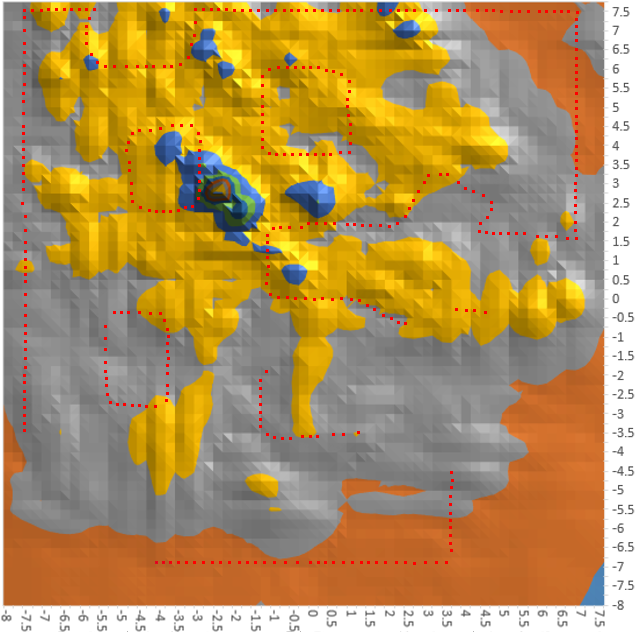
\includegraphics[width=9cm,keepaspectratio]{images/landscape_overlay.png}
	\caption{Fitness maxima corresponding to the position from where the scan was taken. (see \autoref{fig:scan110} for scan and pose positions)}
	\label{fig:landscape}
\end{figure}

\section{Parameter optimisation}
\subsection{Population \& Generations}
As expected, allowing the algorithm to evolve a larger population with/or for a larger number of generations provides improvements to the fitness of the solution provided. However, these require an impractically large computational power: as we can see in \autoref{fig:ga_pop_gen}, a simple evolution of 50 generations with a population of 50 requires an average 37 seconds, on a 16 core machine. As the computational power requirements increase linearly with the number of generations and population size, these would become prohibitively expensive to run in a real time environment. As such, evaluating algorithms using a small population and number of generations will also present a difficult challenge for algorithms, allowing the difference in convergence speeds to be accentuated. , whilst also enabling us to run our experiments in a timely manner to compare algorithms. 
\begin{figure}[]
\centering
	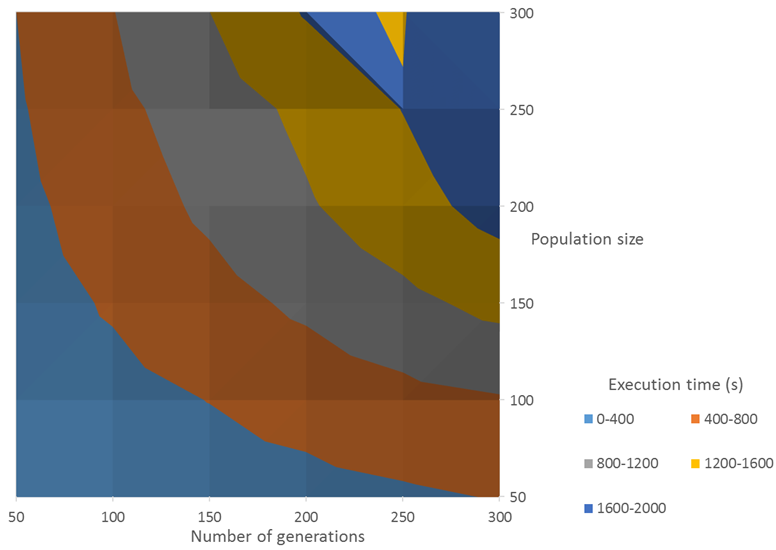
\includegraphics[width=9cm,keepaspectratio]{images/ga_pop_gen_sweep.png}
	\caption{Execution time of the benchmark GA using scan110 and various number of generations and population sizes. (see \autoref{fig:scan110} for scan and pose positions)}
	\label{fig:ga_pop_gen}
\end{figure}

\subsection{Mutation \& Crossover}
\label{subsec:benchmark_mutpb_cxpb}
The mutation and crossover probabilities for our benchmark were found using 60 pose estimations using scan110, our map, and benchmark algorithm with each combination of parameters across a range, as seen in \autoref{fig:ga_cxpb_mutpb}. This high sample number was done to ensure the robustness of the solution, establishing a hard benchmark for our subsequent algorithm comparisons.

\begin{figure}[]
\centering
	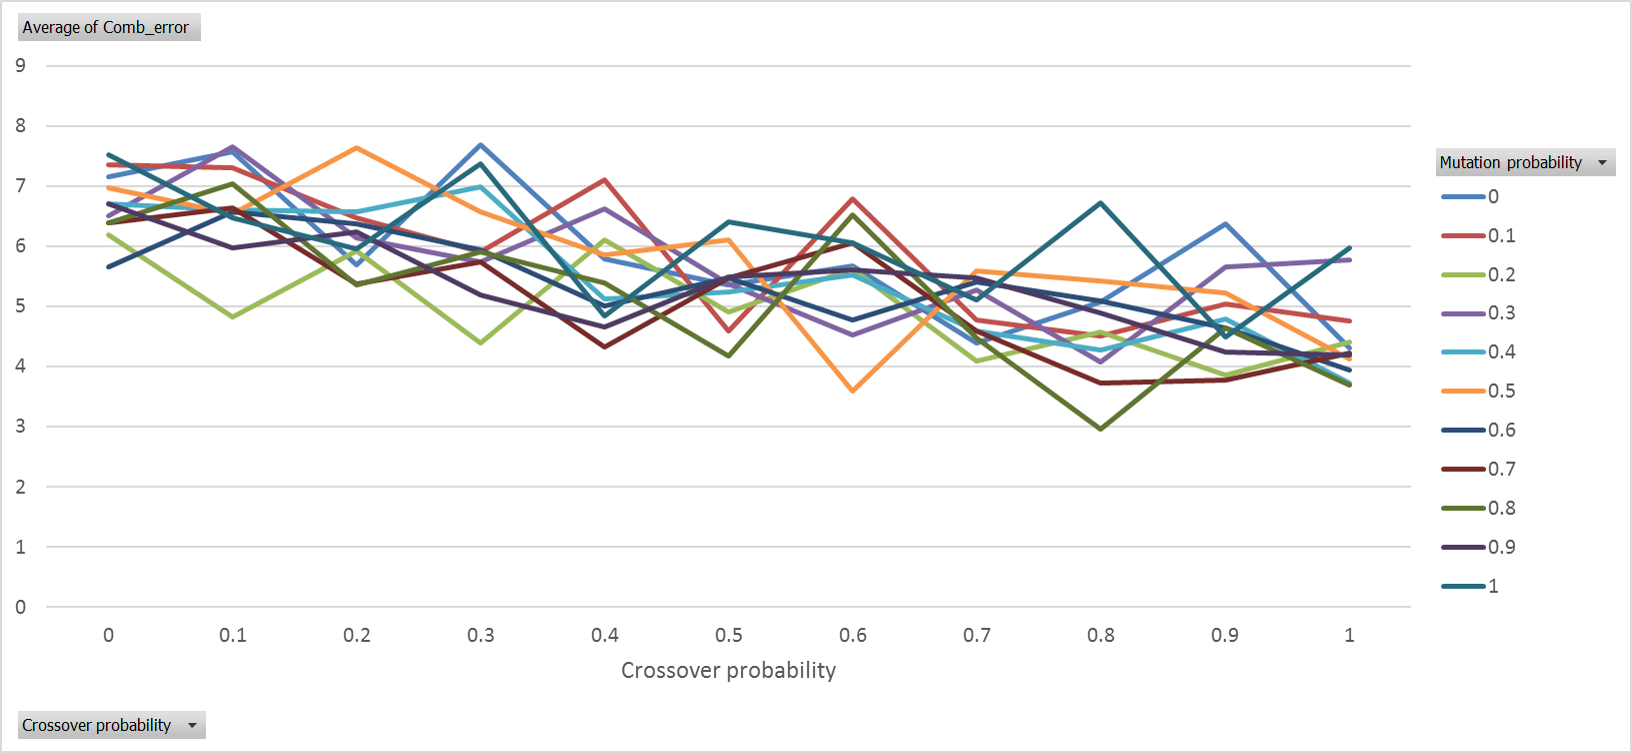
\includegraphics[width=12cm,keepaspectratio]{images/ga_cxpb_mutpb.png}
	\caption[Optimising cross and mutation rate for benchmark algorithm.]{Effects of crossover and mutation rates on the benchmark algorithm's execution time.}
	\label{fig:ga_cxpb_mutpb}
\end{figure}

 This found an apparent optimal parameter set of CXPB=0.8 and MUTPB=0.8. Due to the random nature of genetic algorithms, this does not guarantee a good solution would be found at every run, but allows us some assurance that the average run from the benchmark using these parameters will be the most precise for this algorithm. Due to the variation in scans and maps, it is important to note that these parameters may not be optimal for other scans or maps, but are likely to require tuning through repeated experiments. 

 % [TODO DISCUSS with additional data!!].

\subsection{Mutation size}

\pgfplotstableread[col sep=comma]{data/benchmark/mutsize.csv}\datatablebenchmarkmutsize

\begin{figure}
	\centering
	\begin{tikzpicture}
	    \begin{axis}[
	        xtick=data,
	        % xticklabels from table={\datatableelitemutsize}{mutsize},
	        xticklabel style={rotate=45},
	        width  = 0.8\textwidth,
	        height = 5cm,
	        ylabel = {Combined error},
	        xlabel = {Squared variance of standard distribution from which step sizes are drawn.},
	        ymin=0,
	        xmin=0.2,
	        ymajorgrids=true,
	        % xmax=1.4,
	        % grid=both,
	    ]

	    \addplot+table [col sep=comma, x=mutsize, y=comb_error] {\datatablebenchmarkmutsize};
	    \end{axis}
	\end{tikzpicture}
	\caption[Optimising mutation step size for the benchmark algorithm.]{Effects of varied mutation sizes on performance of the benchmark algorithm.}
	\label{fig:benchmark_mutsize}
\end{figure}

The size of the mutation was defined as a random sample from a normal distribution with $\mu=0, \sigma=1.0$; this was deemed to provide a balance between the frequency in small mutations (to adequately refine the final pose) and larger mutations (to increase the convergence rate of the pose from the initial pose). The near-optimality of this distribution for our test scan (scan 110) was verified by running the algorithm using previously defined parameters and a varying mutation size, as visible in \autoref{fig:benchmark_mutsize}.


\chapter{Algorithm design}
\section{Objectives}
\label{sec:objectives}
The algorithm we aim to implement should improve on existing solutions in the following ways:
\begin{itemize}
	\item Improve the accuracy and precision of the estimated pose
	\item Reduce the computational time required to produce this pose
\end{itemize}
In order to evaluate the relative improvements of our algorithm, we will first re-implement the best existing GA (non-lookup) [AND THEN GLASM?] as follows.

The algorithm aims to achieve the goals defined \autoref{sec:objectives} through a series of independent improvements described in the following sections. These are the use of elitism selection strategies (\autoref{subsec:elitism_sel}) and pre-emptively organising the population of individuals (\autoref{subsec:grid_based_feature}).


\section{Elitism selection}
\label{subsec:elitism_sel}
As seen in the 3d charts of the fitness landscapes seen in \autoref{sec:fitness_landscape}, the fitness of our solutions evolve in a smooth landscape, generally with a significantly larger global maxima. We hypothesised that this would allow us to utilise highly convergent forms of GA's; this was on the assumption that our population was large enough to place one or more individuals in an area such that the individual's local maxima was the global maxima. This individual would then be more likely to have a higher fitness than the rest of the population (due to the smooth fitness landscape), and therefore a high rate of duplication and mutation would enable an evolution towards the global maxima. The concept is built on \citet{David_E_Goldberg1991-es}'s solution to balancing the conflict between exploration and exploitation through higher growth ratios followed by building block discovery through mutation; we however diverge from this by instead utilising mutation to optimise our current local maxima (i.e: block) and assume our initial population was sufficiently dense and spread across the map to find all local maximas.
	
This represented a form of elitism, where the top n percentile of the population was retained at each generation, duplicated into exact offspring, and mutated according to a set probability. \citet{T_Back_D_B_Fogel_T_Michalewicz} and \citet{Shapiro1992-qm} describe an accurately similar algorithm known as the $(\mu + \lambda)$  algorithm.

As with our benchmark algorithm, parameters of the $(\mu + \lambda)$ algorithm were refined using a series of short experiments; these are described in the following sections.

The computational complexity of a fitness-ranked sorting method (quicksort in $O(n log (n))$) is more complex  \cite{Mitchell1998-td} than that of a tournament selection $(O(n))$ \cite{David_E_Goldberg1991-es}, but given the small population size (50) this results in a negligible difference in computational time. This may become an issue when locating in larger maps, which may require larger populations to adequately sample the space for local maximas, but this issue will be secondary to the evaluation time required for each individual.

\subsection{Crossover and Mutation}
\label{subsec:elite_cxpb_mupb}
As with the benchmark algorithms, near-optimal crossover and mutation rates were found by evaluating combinations of these in range (0, 1). Valid combinations are restricted according to $mutpb + cxpb <= 1$, which produces the correct number of offspring at each generation. These combinations were evaluated 30 times each over 50 generations, with a population of 50 individuals and an elitism of 0.8 (that is, the top 80\% of the population are carried over into the next generation and used to produce the next generation's remaining population as offspring). The experiment was initIally conducted using scan110, which we deem to be sufficient as the crossover and mutation rates of the individuals are used in our algorithm to provide pose refinement rather than increase the breadth of search; as maps can be expected to have a smooth peak (as seen in the fitness landscapes in \autoref{sec:fitness_landscape}), the mutation and crossover rates are expected to be near-optimal for most scans in the map. To increase our confidence in this assumption, an equivalent search was conducted on a randomly selected scan (scan64) as seen below.

% FROM elitism/CXPB_ga_elite.xslx
\begin{figure}
\begin{subfigure}[b]{0.5\textwidth}
	\resizebox{\linewidth}{!}{
		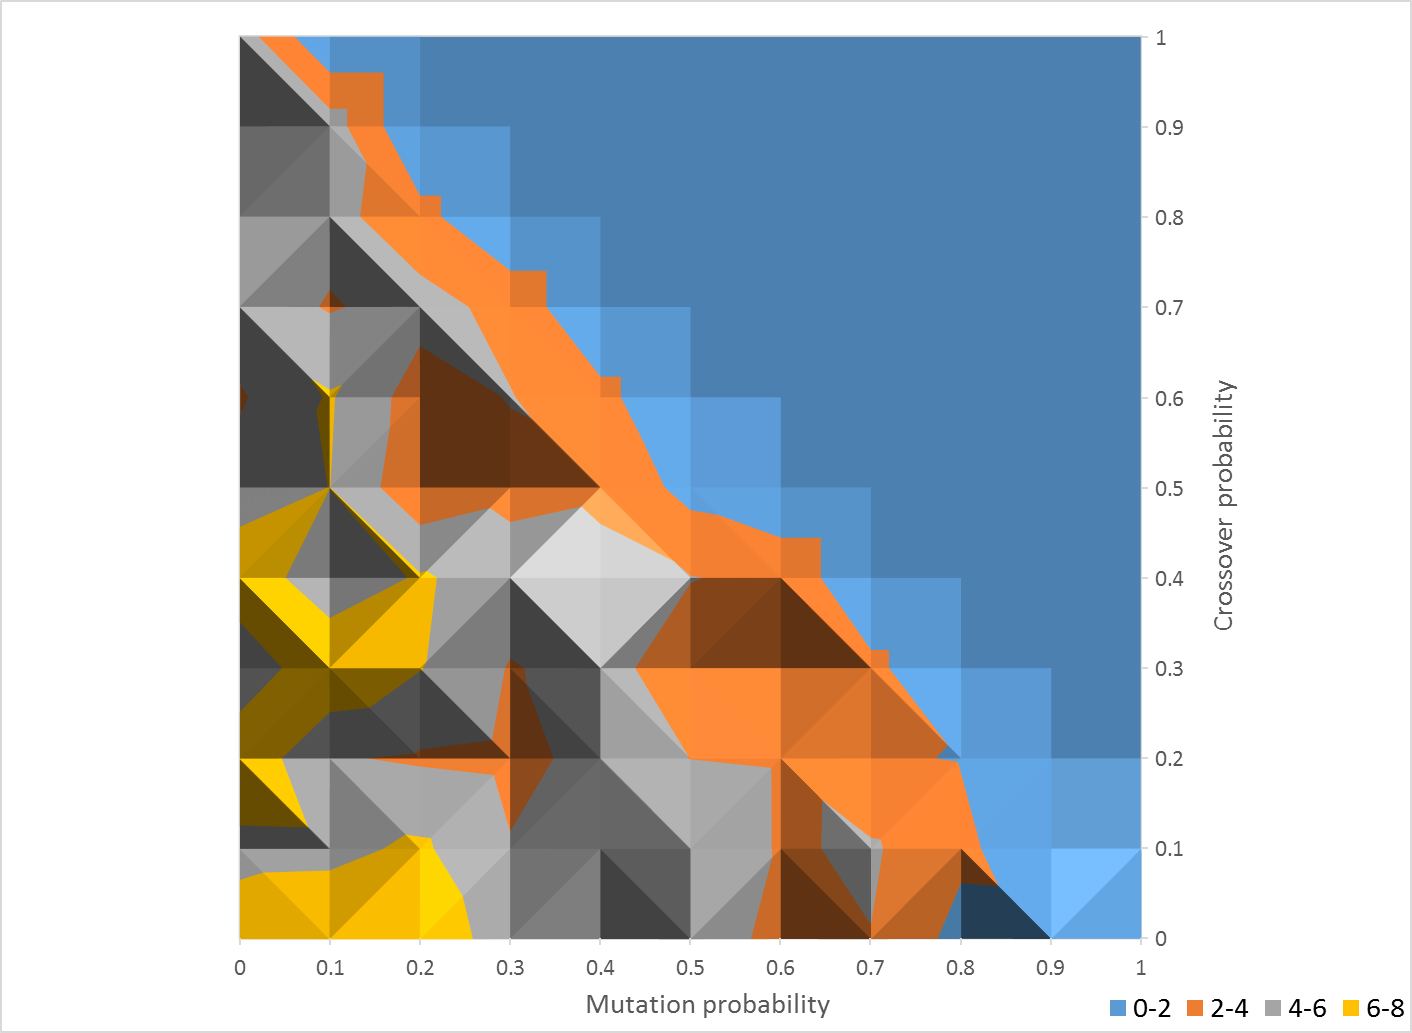
\includegraphics[width=9cm,keepaspectratio]{images/ga_elite_cxpb_mutpb110.png}
	}
\end{subfigure}
\begin{subfigure}[b]{0.5\textwidth}
	\resizebox{\linewidth}{!}{
		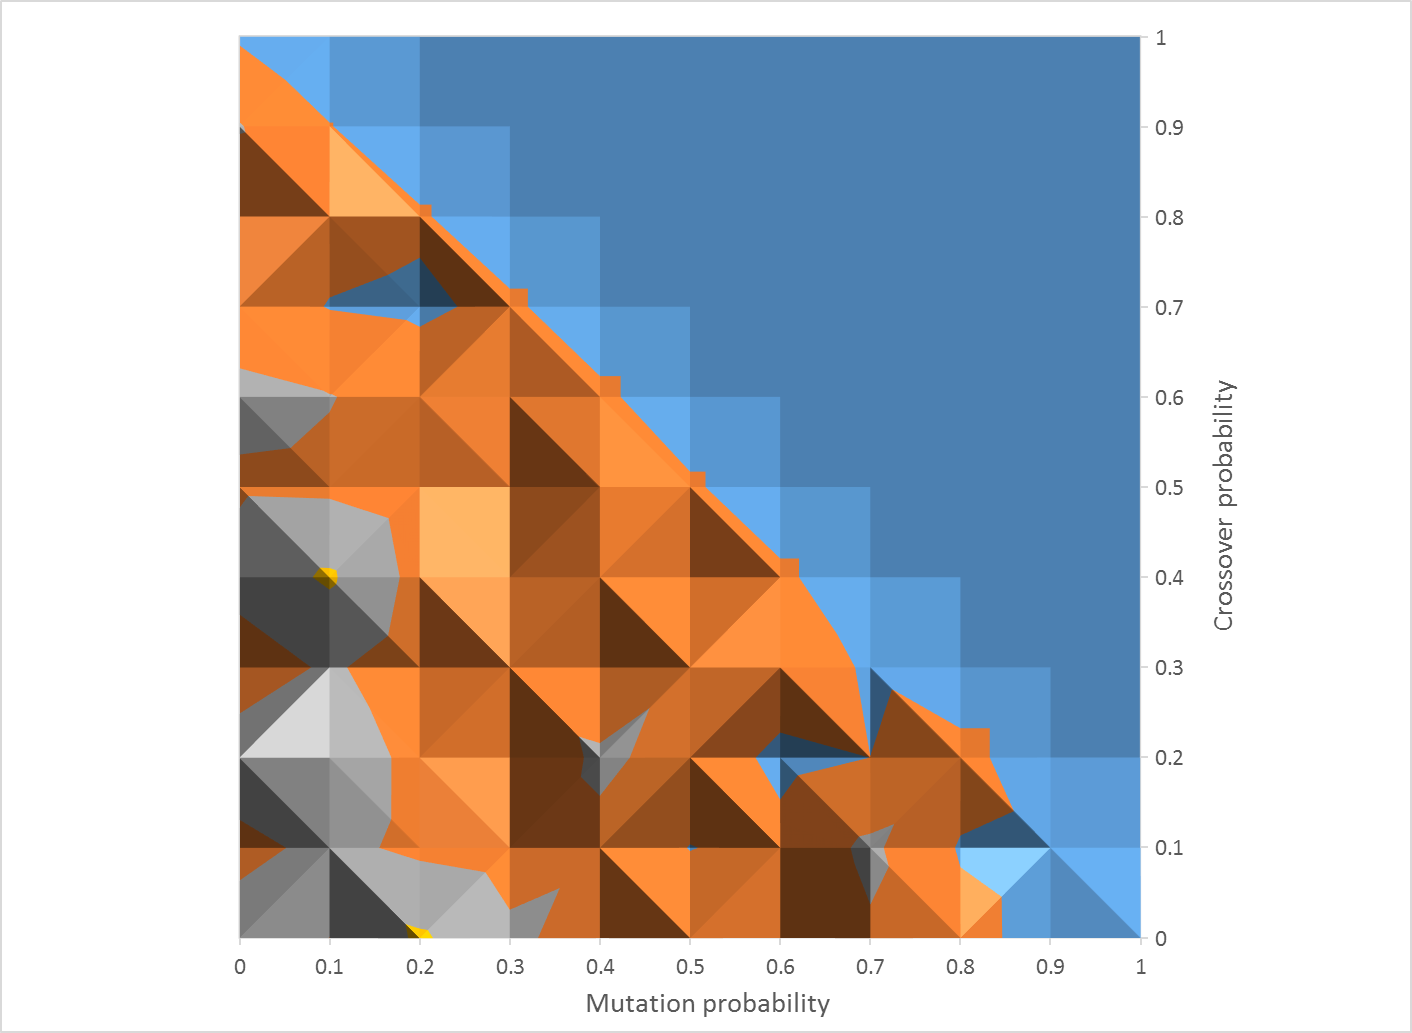
\includegraphics[width=9cm,keepaspectratio]{images/ga_elite_cxpb_mutpb64.png}
	}
\end{subfigure}
	\caption[Optimising crossover \& mutation rates for elitist selection.]{Effects of crossover and mutation rates on the benchmark algorithm's average combined error, using scan110 (left) and scan64 (right).}
	\label{fig:ga_elite_cxpb_mutpb_exec_time}
\end{figure}

This resulted in \autoref{fig:ga_elite_cxpb_mutpb_exec_time}, which demonstrates that an average minimal combined error will occur when utilising a 100 \% mutation rate and no crossover; we will therefore use as the basis for which to select further parameters. This result can be explained by the fact that it maximises the movement of an individual throughout the evolution. Individuals which randomly move towards maximas are maintained in the population (as they will have a higher fitness), whilst individuals which distance themselves from the maxima sufficiently (and therefore a lower fitness) will eventually be removed from the population by the elitism.


\subsection{Elitism rate}
\label{subsec:elite_elitism_rate}
Corresponding elitism rates were selected using another exhaustive search from $0 <= n <= 1$, where n represents the top percentage of candidate poses which are kept for the next generation. This feature would affect the trade-off between the breadth of search (as does the population size), and the speed of convergence of the algorithm (as worse solutions are more rapidly removed from the population). We expect the optimal elitism rate to be strongly affected by the smoothness of the fitness landscape: maps with multiple peaks in fitness (i.e: a scan strongly matches multiple features in the map) may require a slower convergence to ensure they find the global maxima, whilst a faster convergence rate (by selecting fewer individuals at each generation) could allow poses in smoother maps to be quickly found. In order to find a near-optimal elitism rate, 30 evaluations of the algorithm with varying elitism rates were ran using Scan110 and our reference map, in addition to the previously established mutation and crossover rates.

% from elite_sweep_110(latest)
\begin{figure}
	\centering
	\begin{tikzpicture}
	    \begin{axis}[
	        xtick = {0.1, 0.2, 0.3, 0.4, 0.5, 0.6, 0.7, 0.8, 0.9, 1.0},
	        width  = \textwidth,
	        height = 8cm,
	        ylabel = {Combined error},
	        xmin = 0,
	        ymin=0,
	        xmax=1.05,
	        ymax=14,
	        grid=both,
	        xlabel = {Proportion of top individuals selected.},
	        legend pos=north east,
	        legend columns = 4,
	    ]
	    \addplot+ table [col sep=comma, x=elitism, y=scan2] {data/elite/elitism.csv};
	    \addlegendentry{Scan2}

	    \addplot+ table [col sep=comma, x=elitism, y=average] {data/elite/elitism.csv};
	    \addlegendentry{Average}

	    \addplot+ table [col sep=comma, x=elitism, y=scan64] {data/elite/elitism.csv};
	    \addlegendentry{Scan64}

	    \addplot+ table [col sep=comma, x=elitism, y=scan110] {data/elite/elitism.csv};
	    \addlegendentry{Scan110}
	    \end{axis}
	\end{tikzpicture}
	\caption[Optimsing elitism rate for scan/map]{Effecs of elitism rate on combined error.}
	\label{fig:elitsm_rates}
\end{figure}
As we can see in the figure above, there appears to be an optima at 0.95 (95\% of the population is maintained and mutated into the next generation whilst 5\% are produced), which indicates the need for a slower convergence than we expected. This is the case for both scan110 and the average of scans 2, 64 and 110, and will therefore be used when evaluating our algorithm in our benchmark.

% TODO discuss further

\subsection{Mutation size}

\pgfplotstableread[col sep=comma]{data/elite/mutsize.csv}\datatableelitemutsize

\begin{figure}
	\centering
	\begin{tikzpicture}
	    \begin{axis}[
	        xtick=data,
	        % xticklabels from table={\datatableelitemutsize}{mutsize},
	        xticklabel style={rotate=45},
	        width  = 0.8\textwidth,
	        height = 5cm,
	        ylabel = {Combined error},
	        xlabel = {Squared variance of standard distribution from which step sizes are drawn.},
	        ymin=0,
	        xmin=0.2,
	        ymajorgrids=true,
	        % xmax=1.4,
	        % grid=both,
	    ]

	    \addplot+table [col sep=comma, x=mutsize, y=comb_error] {\datatableelitemutsize};
	    \end{axis}
	\end{tikzpicture}
	\caption[Optimising mutation step size for the elitist selection algorithm.]{Effects of varied mutation sizes on performance of the elitist algorithm.}
	\label{fig:elite_mutsize}
\end{figure}

The size of the mutation was defined as a random sample from a normal distribution with $\mu=0, \sigma=1.05$; this was deemed to provide a balance between the frequency in small mutations (to adequately refine the final pose) and larger mutations (to increase the convergence rate of the pose from the initial pose). The near-optimality of this distribution for our test scan (scan 110) was verified by running the algorithm using previously defined parameters and a varying mutation size, as visible in \autoref{fig:elite_mutsize}.




\subsection{Evaluation against Benchmark}
\subsubsection{Balanced population size and number of generations}
\label{subsec:ga_vs_elite_eq_pop_gen}
The algorithm was first compared to a benchmark using an equal population size and number of generations. This was evaluated 30 times using optimal parameters for each algorithm, using scan110 as a representative of scans in the dataset. This found that our elitist algorithm was capable of finding more precise poses with limited algorithmic capacity, with a mean combined error of 0.191 against 1.839. The result was validated using a two-tailed T-Test (with unequal variance) between the set of combined errors (N=30, p<0.01). However, the elitist algorithm also required slightly more time to run, which brings into question the efficacy of the algorithm when implemented on target.

% From elite/Elite_vs_GA.xslx
\begin{table}
\centering
\begin{tabular}{|l|l|l|l|l|}
\hline & \multicolumn{2}{l|}{\textbf{Combined error}} & \multicolumn{2}{l|}{\textbf{Execution time (s)}} \\ \hline & 
\textbf{Benchmark} & \textbf{Elitism}& \textbf{Benchmark}   & \textbf{Elitism}  \\ \hline 
\textbf{Mean} & 1.839   & 0.191  & 46.923 & 48.522  \\ \hline
\textbf{Stdev}  & 3.151   & 0.478 & 9.160 & 9.057 \\ \hline
\end{tabular}
\caption[Effects of elitist against tournament selection (table)]{Combined error and execution time over 30 runs of benchmark and elitist algorithms}
\label{tab:ga_vs_elite_eq_pop_gen}
\end{table}

\subsubsection{Equal execution time}
\label{subsec:ga_vs_elite_time_sweep}
Further to the previous experiment, the code was modified to loosely constrain the available execution time; this functioned by halting the algorithm if, at the end of a generation, the elapsed time was larger than a specified threshold. As the subsequent results functioned in unequal execution times, the results were weighed according to their execution time, such that the statistics were ran on values representing the product of the execution time and combined error. A lower value is therefore preferable as it indicates the algorithm was either more precise than the other given a certain computational time, required less computational time to produce an equally precise result, or a combination of the two. 

This produced the data visible in \autoref{fig:ga_vs_elite_box_whiskers}; as we can see, the elite algorithm produces more efficient results across the set of target execution times. This is most visible by the comparatively low median (0.550 against 12.960), along with a more efficient upper quartile (2.110 against 82.407). This demonstrates that the elite algorithm produces consistently more efficient solutions than the benchmark algorithm. It does however either take an excessively long period of time or produces poor results, as demonstrated by the large whiskers (this is addressed in \autoref{subsec:grid_based_feature}).


% From elitism/elite-vs_ga
\begin{figure}
	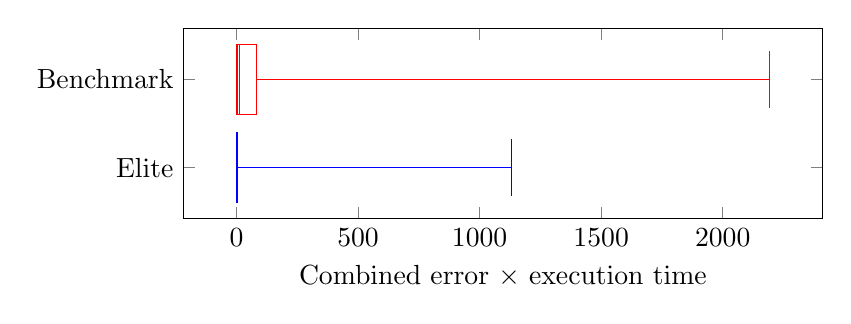
\begin{tikzpicture}
		\begin{axis}
		[height=4cm, width=0.8\textwidth, ytick={1,2}, yticklabels={Elite, Benchmark}, xlabel={Combined error $\times$ execution time}]

		\addplot+[
			boxplot prepared={
				median = 0.549995769,
				upper quartile = 2.110914904,
				lower quartile = 0.218344227,
				upper whisker = 1130.260711,
				lower whisker = 2.34E-05,
			},
		] coordinates {};	

		\addplot+[
			boxplot prepared={
				median = 12.96005201,
				upper quartile = 82.40675284,
				lower quartile = 2.282474981,
				upper whisker =  2191.115298,
				lower whisker = 0.000318737,
			},
		] coordinates {};
		\end{axis}
	\end{tikzpicture}
	\caption[Effects of elitist against tournament selection (box-plot)]{Performance of each algorithm with 50 population, as many generations as possible within the time frame and optimal parameters for each algorithm.}
	\label{fig:ga_vs_elite_box_whiskers}
\end{figure}

These results can be further analysed in \autoref{fig:ga_vs_elite_bucket}, where the results are grouped into buckets of execution time. A bucket-paired T-Test demonstrates the results from the elite algorithm are statistically more efficient (i.e: execution time $\times$ combined error is lower) per execution time (means of 23.622 vs 100.865, p<0.001, N=360). This is not the case for all time limits; benchmark runs limited to 5-10s are not significantly more efficient (23.724 average combined error $\times$ execution time) than the elite algorithm (26.231). This may be due to the benchmark's use of crossovers to rapidly explore areas of the map which are not yet populated; an equivalent breadth of search is not available in our algorithm due to the small mutation sizes and lack of crossover, which we will address in our next feature in \autoref{subsec:grid_based_feature}. 

We can also notice that the precision per time unit seems to increase as we provide the elite algorithm with additional time, leading to an exponential decrease in error. In contrast, the benchmark algorithm appears to follow a constant efficiency. 

\pgfplotstableread[col sep=comma]{data/ga_vs_elite/time_limited_buckets.csv}\datatable
\begin{figure}
	\centering
	\begin{tikzpicture}
	    \begin{axis}[
	        ybar,
	        axis y line*=left,
	        xtick=data,
	        xticklabels from table={\datatable}{bucket},
	        xticklabel style={rotate=45},
	        bar width=0.2,
	        % bar shift=0pt,
	        grid=both,
	        width  = \textwidth,
	        height = 5cm,
	        ylabel = {Execution time $\times$ combined error},
	        xlabel = {Real execution time (s)},
	        % scaled y ticks = false,
	        legend pos = north west,
	        ymax=450,
	        ymin=0,
	    ]
	    \addplot+[fill opacity=0.75] table [col sep=comma, x expr=\coordindex, y=elite_errortime, fill opacity=0.5] {data/ga_vs_elite/time_limited_buckets.csv};

	    \addplot+[fill opacity=0.5] table [col sep=comma, x expr=\coordindex, y=benchmark_errortime, fill opacity=0.5] {data/ga_vs_elite/time_limited_buckets.csv};
	    \addlegendentry{Elite time $\times$ error}
	    \addlegendentry{Benchmark time $\times$ error}
	    \end{axis}

	    \begin{axis}[
	    	axis y line*=right,
	        xtick=data,
	        xticklabels from table={\datatable}{bucket},
	        xticklabel style={rotate=45, opacity=0.0},
	        width  = \textwidth,
	        height = 5cm,
	        ylabel = {Combined error},
	        ymax=12,
	        ymin=0,
	    ]
	    \addplot+table [col sep=comma, x expr=\coordindex, y=elite_error] {data/ga_vs_elite/time_limited_buckets.csv};
	    \addplot+table [col sep=comma, x expr=\coordindex, y=benchmark_error] {data/ga_vs_elite/time_limited_buckets.csv};
	    \addlegendentry{Elite error}
	    \addlegendentry{Benchmark error}

	    \end{axis}
	\end{tikzpicture}
	\caption[Effects of elitist against tournament selection (bar-line chart)]{Average run time $\times$ combined error for each algorithm, using as many generations as possible in time limit, optimal parameters for each algorithm and population of 50.}
	\label{fig:ga_vs_elite_bucket}
\end{figure}

As demonstrated in \autoref{subsec:ga_vs_elite_time_sweep}, fitness-rank based selection is capable of rapidly selecting promising individuals, duplicating them and mutating their offspring to find an optima near them. This results in an algorithm which is more efficient in a majority of time scales, but can still fail to produce a precise pose given an arbitrary amount of computational time (as demonstrated by the larger upper whisker in \autoref{fig:ga_vs_elite_box_whiskers}). This may be due to the stochastic nature of the genetic algorithms, or more particularly the population initialisation. 

Whilst the benchmark algorithm has an equally large worst case, we can hypothesise that this is due to the inability of the algorithm to evolve it's poses with sufficient precision. In contrast, the elite algorithm's duplication and mutation of individuals increases the number of local explorations around existing individuals, but is incapable of evaluating areas which were not populated by the initial population. This has led to the development of a grid-based initial population, as detailed in \autoref{subsec:grid_based_feature}.

\subsection{Grid-based initial population}
\label{subsec:grid_based_feature}
 As previously stated, rank-based selection of individuals causes the algorithm to be unable to explore areas which were not sampled in the initial population. It would be possible to increase the probability of sampling every area in the map by increasing the population size, but this would lead to a larger execution time as a certain number of generations may still be required to sufficiently refine the position of an individual via duplication and mutation, even if the required displacement is reduced by the increased population density.

 In order to provide an adequate breadth of search without a large computational overhead, we utilised a simple algorithm to place a set number of individuals in a map at a constant density; this is visible by the red dots in \autoref{fig:grid_init} which represent individuals in the map. This enabled the algorithm to initially evaluate a larger number of 'candidate' individuals, of which 50 are selected and mutated to begin the previous evolution; this action forms the first generation of our algorithm. Subsequent generations are the same as in the non-grid algorithm. 

\begin{figure}[ht]
\centering
	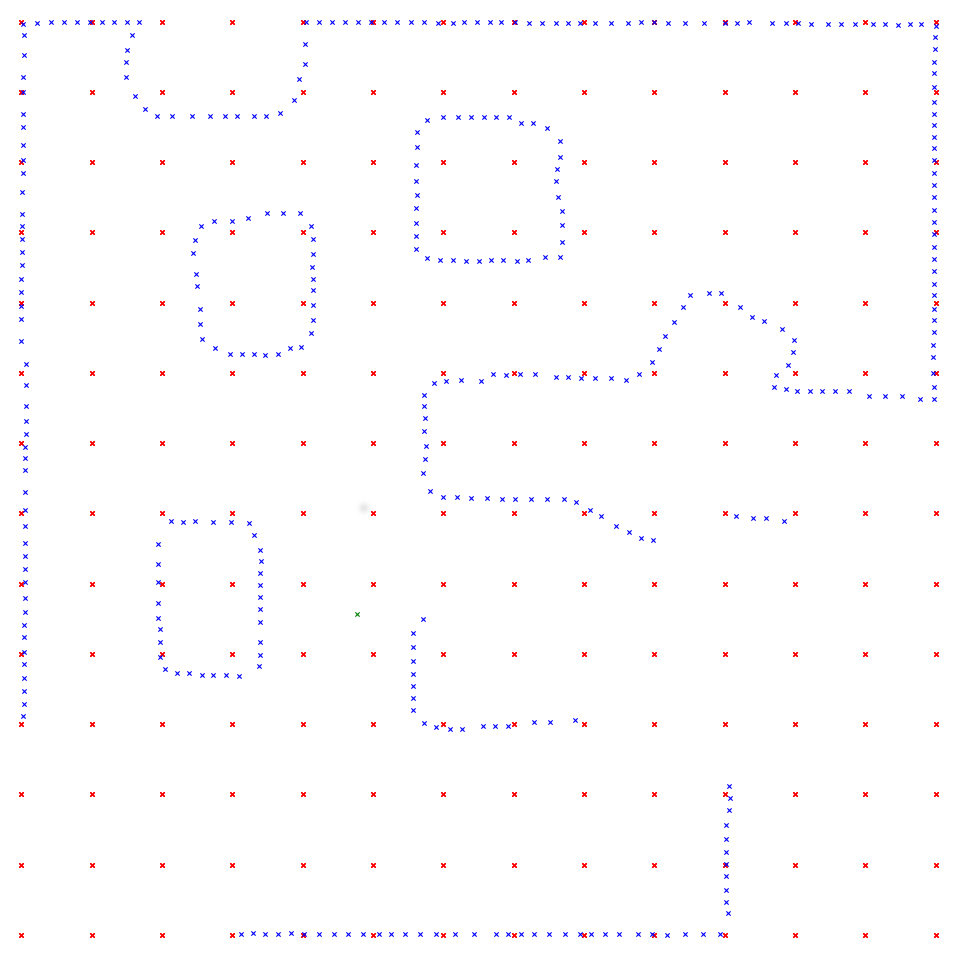
\includegraphics[width=4cm,keepaspectratio]{images/grid.png}
	\caption{A grid based initial population}
	\label{fig:grid_init}
\end{figure}

The effects of pre-arranging a larger population were evaluated using the same methodology with which our algorithm was previously compared to the benchmark. The elitist algorithm including a grid-based initialisation of 200 individuals (followed by the evolution of the 50 best individuals) was executed 30 times across a range of time limits, producing the data found in \autoref{fig:grid_vs_elit}. 

\pgfplotstableread[col sep=comma]{data/rand_vs_grid/timesweep.csv}\datatablegrid

\begin{figure}
	\centering
	\begin{tikzpicture}
	    \begin{axis}[
	        ybar,
	        axis y line*=left,
	        xtick=data,
	        xticklabels from table={\datatablegrid}{bucket},
	        xticklabel style={rotate=45},
	        bar width=0.2,
	        grid=both,
	        % bar shift=0pt,
	        width  = \textwidth,
	        height = 7cm,
	        ylabel = {Execution time $\times$ combined error},
	        xlabel = {Real execution time (s)},
	        ymin=0,
	        ymax=170,
	        % scaled y ticks = false,
	        legend pos = north west
	    ]
	    \addplot+[fill opacity=0.75] table [col sep=comma, x expr=\coordindex, y=rand_errortime, fill opacity=0.5] {\datatablegrid};
	    \addplot+[fill opacity=0.75] table [col sep=comma, x expr=\coordindex, y=grid_errortime, fill opacity=0.5] {\datatablegrid};

	    \addlegendentry{Elite time $\times$ error}
	    \addlegendentry{Grid time $\times$ error}
	    
	    \end{axis}

	    \begin{axis}[
	    	axis y line*=right,
	        xtick=data,
	        xticklabels from table={\datatablegrid}{bucket},
	        xticklabel style={rotate=45, opacity=0.0},
	        width  = \textwidth,
	        height = 7cm,
	        ylabel = {Combined error},
	        ymax=1.5,
	        ymin=0,
	    ]
	    \addplot+table [col sep=comma, x expr=\coordindex, y=rand_error] {\datatablegrid};
	    \addplot+table [col sep=comma, x expr=\coordindex, y=grid_error] {\datatablegrid};
	    \addlegendentry{Elite error}
	    \addlegendentry{Grid error}
	    \end{axis}
	\end{tikzpicture}
	\caption[Benefit of grid-based initialisation.]{Performance of grid-based initialisation compared to elitist algorithm.}
	\label{fig:grid_vs_elit}
\end{figure}

Using the same TTest (paired across bucketed real execution time) we found the mean efficiency to be statistically lower for grid-initialised algorithms (with a larger initial population which is later reduced) as opposed to standard initialisations (average execution time $\times$ error of 2.26 vs 69.00, p<0.001, N=360). This is likely due to a reduction in the number of algorithm failures, where no adequate pose was found within the time limit. This can be seen in \autoref{fig:grid_vs_rand_stdev}, where the standard deviations for each execution time group are generally lower for grid-based initialisation than the standard algorithm. This is found to be statistically significant for two thirds of the groups using an F-Test (p<0.001), therefore demonstrating that grid-based initialisations greatly increase the precision of the algorithm. We should note that optimal grid density or parameters were not explored for the map or scan, and it could therefore be possible to further accentuate the effect of this method on the output pose.

\pgfplotstableread[col sep=comma]{data/rand_vs_grid/stdev.csv}\datatablegridstdev

\begin{figure}
	\centering
	\begin{tikzpicture}
	    \begin{axis}[
	        xtick=data,
	        xticklabels from table={\datatablegridstdev}{buckets},
	        xticklabel style={rotate=45},
	        width  = 0.8\textwidth,
	        height = 5cm,
	        ylabel = {Combined error stdev},
	        xlabel = {Real execution time (s)},
	        ymin=0,
	        grid=both,
	    ]
	    \addplot+table [col sep=comma, x expr=\coordindex, y=grid_stdev] {\datatablegridstdev};
	    \addplot+table [col sep=comma, x expr=\coordindex, y=rand_stdev] {\datatablegridstdev};
	    \addlegendentry{Grid initialisation}
	    \addlegendentry{Standard initialisation}
	    \end{axis}
	\end{tikzpicture}
	\caption[Grid vs. random population layout]{Improved pose accuracy and algorithm success from grid-based initialisations compared to random initialisation.}
	\label{fig:grid_vs_rand_stdev}
\end{figure}

We should additionally note that while the feature was envisioned using a grid-like pattern, the use of a larger initial population which is randomly distributed around the map does achieve similarly distinct results when compared to the elitist algorithm. This was validated over 30 runs of the algorithm, which produced a mean result (in execution time $\times$ combined error) of 3.74 across all execution time buckets, compared to the grid-based algorithm's mean of 2.255. A paired T-test across execution time buckets does confirm it is not significantly worse than a grid-based initialisation (N=360, p=0.295).

\begin{figure}
	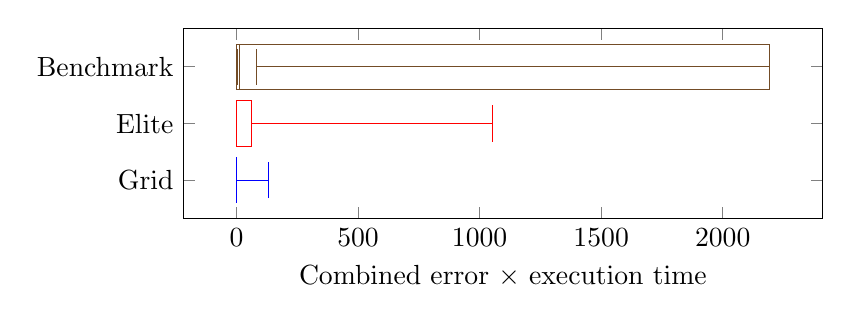
\begin{tikzpicture}
		\begin{axis}
		[height=4cm, width=0.8\textwidth, ytick={1,2, 3}, yticklabels={Grid, Elite, Benchmark}, xlabel={Combined error $\times$ execution time}]

		\addplot+[
			boxplot prepared={
				median = 0.318204416,
				upper quartile =  0.853609313,
				lower quartile =  0.101603705,
				upper whisker = 131.3713864,
				lower whisker = 0.001041047,
			},
		] coordinates {};	

		\addplot+[
			boxplot prepared={
				median = 1.833061726,
				upper quartile =  63.10291318,
				lower quartile =  0.247805344,
				upper whisker =  1053.747935,
				lower whisker = 0.00002342,
			},
		] coordinates {};

		\addplot+[
			boxplot prepared={
				median = 12.96005,
				upper quartile = 2191.115,
				lower quartile = 0.000319,
				upper whisker = 82.40675,
				lower whisker = 2.282475,
			},
		] coordinates {};
		\end{axis}
	\end{tikzpicture}
	\caption[Grid, Elitism, Benchmark time-adjusted performance.]{Performance of each algorithm over 30 executions for various time limits.}
	\label{fig:ga_vs_elite_vs_grid_box_whiskers}
\end{figure}

As such, 'primed' populations of individuals are hugely beneficial to the evolution of a pose through elitism selection, as they increase the probability that an individual will be placed in a position from which it would crawl (via mutation and duplication) towards the global maxima. This addition further contributes to improving the consistency of pose retrieval, as well as reducing the worst case pose, as demonstrated by the compact box plot representing the Grid algorithm's results in \autoref{fig:ga_vs_elite_vs_grid_box_whiskers}.




% Evaluate over large dataset, measure success rate?

\chapter{Experimental summary \& Conclusion}
In this report we have examined the effects of elitist selection and population priming on the precision and computational time of genetic algorithms, within the context of indoor localisation using Cartesian data. Experiments detailing the variations in result accuracy, precision and computational efficiency were conducted using a feature-dense scan from \citet{Lenac2011-co}, providing a complex comparison between algorithms. 

\section{Elitist selection}
As summarised in \autoref{fig:ga_vs_elite_bucket}, our first experiment showed that a large improvement in efficiency could be obtained from elitist algorithms when executing the algorithm for more than 15 seconds; this allowed the poses to be sufficiently refined via incremental mutation. The elite algorithm was ineffective when unable to evolve for fewer generations, as the lack of a crossover mutation limited the distance covered by generation-iterative random walking. This could be amended by priming the population of individuals or utilising larger mutation sizes, as explored in the grid initialisation experiments and variable mutation rate experiment.

\section{Grid-based initial populations}
The grid-initialisation aimed to improve the global search of the elitist algorithm without significantly increasing the computational requirements of the algorithm. This was achieved by using a larger initial population of candidate poses, evenly distributed over the map. Following a single generation with this larger population, the subsequent evolution took place on the 50 best individuals from that generation (as selected by the fitness function). This resulted in an improved precision, as it increased the likelihood of an individual in the initial population being placed within close proximity of a global maxima (towards which it can mutate). In combination with a small increase in computational time, this lead to a more efficient algorithm across all execution times (as visible in \autoref{fig:grid_vs_elit}). We can safely assume that this would require slightly more memory, due to the increased codebase and larger initial population; this may impede it's implementation in resource-limited systems. 

As previously cited in \autoref{subsec:ICP}, \citet{Censi2005-iv} states that it would be possible to apply a 'classical' algorithm to a global pose localisation problem by running it from a number of random poses. This would rely on the assumption that one of these random poses has a local maxima which is the global maxima; that is, it will be capable of using gradient ascent to refine it's pose, similarly to the methodology implemented by grid-based initialisation. However, ICP remains an extremely efficient algorithm, whilst the mutation-based refinement of a genetic algorithm is more similar to a random walk than a hill climbing algorithm. We have therefore opted to create a basic implementation of an ICP-based algorithm to demonstrate this.

\subsection{ICP algorithm design \& evaluation}
\label{subsec:icp_benchmark}
An ICP algorithm based off the implementation from [STACKOVERFLOW] was adapted for use with our grid-layout algorithm. It functioned by running 20 iterations of the ICP algorithm from 200 hypothetical poses laid across a grid on the map. The pose with the lowest error is then selected using the same error function used in the fitness metric for the GA's. This was executed 360 times to create a set of data comparable to the grid-based algorithm's dataset (which was created using 30 runs over 12 target durations), which was illustrated in \autoref{fig:icp_vs_elite_vs_grid_box_whiskers}. 

As we can see, the global-ICP has a similar median to the grid-based initialisation (medians: Grid = 0.73, ICP = 1.33), but is much more consistent; this is demonstrated by the standard deviation (Grid = 68.63, ICP = 7.760). A paired T-Test across ICP's pose error $\times$ execution time results and the equivalent results from the range of executions of the grid-initialised algorithms found the means to be significantly different (N=360, p<0.001), indicating that the global ICP algorithm is indeed more efficient. In addition, a paired T-Test on the combined pose error (regardless of execution time) found the mean of the ICP algorithm's output to be significantly lower than that of the grid algorithm (N=360, p<0.01, means are: Grid = 16.95, ICP = 1.204). 

Compounding this information with the fact the longest global-ICP execution required 6.7 seconds (mean of 3.66) demonstrates that even an extremely basic and unrefined adaptation of a classic localisation algorithm could out-perform a GA (the classic algorithm could be further improved by fine tuning the density of the initial grid, or utilising an improved version of ICP such as mbICP or trICP).

We will explore the reasons behind this gap in \autoref{sec:algorithm_limitations}



\begin{figure}
	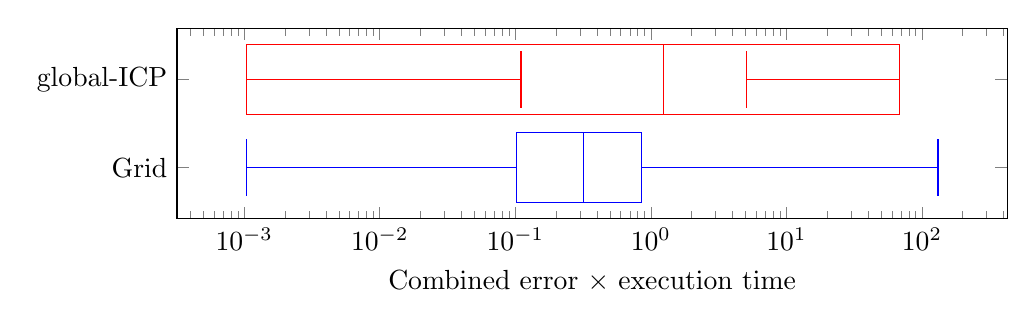
\begin{tikzpicture}
		\begin{axis}
		[height=4cm, width=\textwidth, ytick={1,2, 3}, yticklabels={Grid, global-ICP}, xlabel={Combined error $\times$ execution time}, xmode=log]

		\addplot+[
			boxplot prepared={
				median = 0.318204416,
				upper quartile =  0.853609313,
				lower quartile =  0.101603705,
				upper whisker = 131.3713864,
				lower whisker = 0.001041047,
			},
		] coordinates {};	

		% \addplot+[
		% 	boxplot prepared={
		% 		median = 1.715260273, 
		% 		upper quartile = 60.35376507,
		% 		lower quartile = 0.296903234,
		% 		upper whisker = 1130.260711,
		% 		lower whisker = 0.000817614
		% 	},
		% ] coordinates {};


		\addplot+[
			boxplot prepared={
				median = 1.236822,
				upper quartile = 68.64869,
				lower quartile = 0.001034,
				upper whisker = 5.075329,
				lower whisker = 0.110132,
			},
		] coordinates {};
		\end{axis}
	\end{tikzpicture}
	\caption[Global-ICP performance against Grid Initialisation] {Performance of each algorithm over 30 executions for 12 time limits (note: x axis is logarithmic)}
	\label{fig:icp_vs_elite_vs_grid_box_whiskers}
\end{figure}






\section{Limitations of the algorithm}
\label{sec:algorithm_limitations}
A number of issues could cause the under-performance of the genetic algorithms; these are the fitness function \& the algorithm's inability to fully explore map topology.

\subsection{Fitness function}
The fitness function may be a source of some inaccuracy. \autoref{fig:landscape_peaks} illustrate a high-granularity visualisation of the fitness functions observed in \autoref{fig:landscape} for scan110, demonstrating that the peak of the fitness function does not match the expected pose provided by the Player-Stage model used in \citet{Lenac2011-co}(-2.184327, 2.641909). Instead, a peak further to the north west is indicated by the concentric circles forming a summit. Therefore, we can assume a translation error is due to individuals being caused by the fitness function. This occurs across all 3 sampled tolerance sizes, suggesting it may be specific to this map, scan and pose.

\begin{figure}
\begin{subfigure}[b]{0.3\textwidth}
	\resizebox{\linewidth}{!}{
		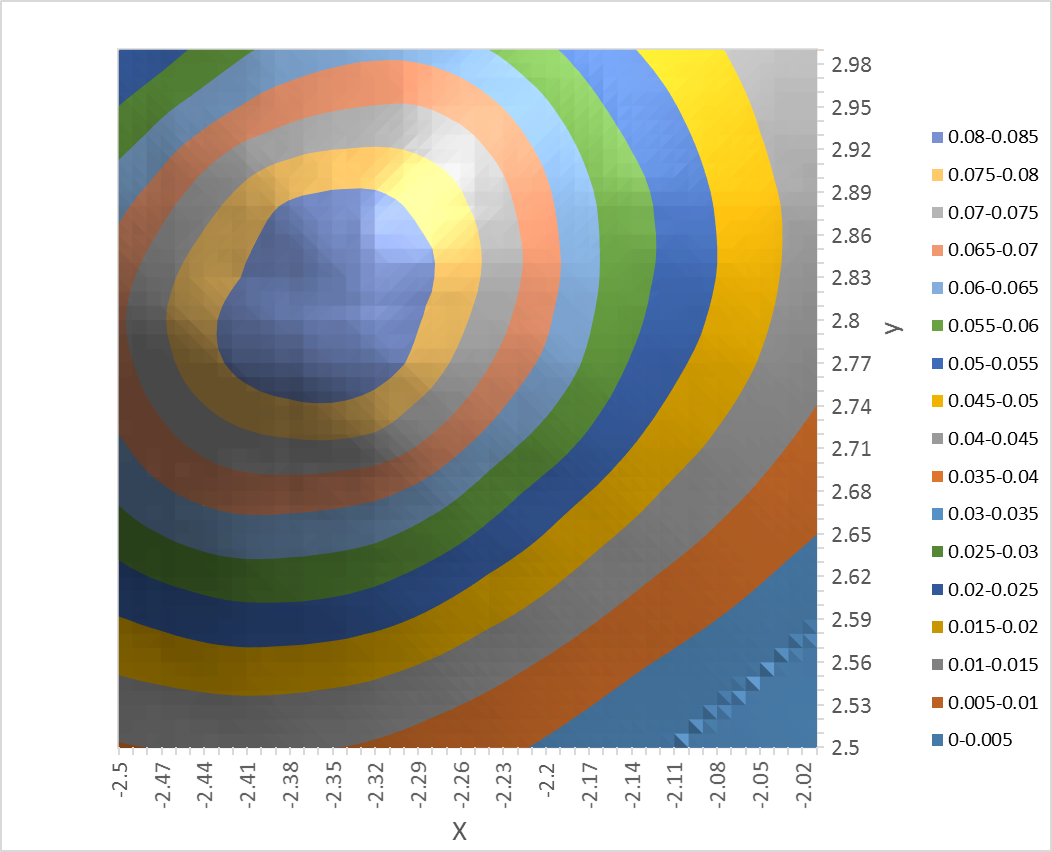
\includegraphics[width=9cm,keepaspectratio]{images/landscape_0_1.png}
	}
\end{subfigure}
\begin{subfigure}[b]{0.3\textwidth}
	\resizebox{\linewidth}{!}{
		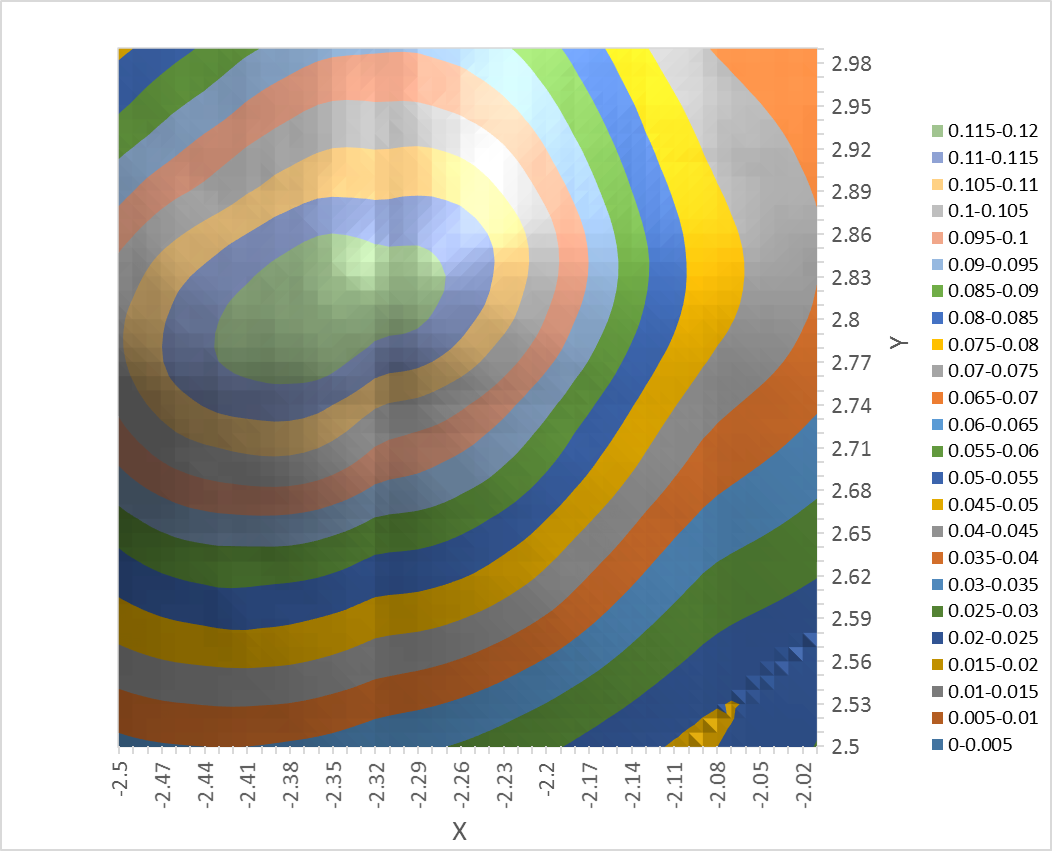
\includegraphics[width=9cm,keepaspectratio]{images/landscape_0_2.png}
	}
\end{subfigure}
\begin{subfigure}[b]{0.3\textwidth}
	\resizebox{\linewidth}{!}{
		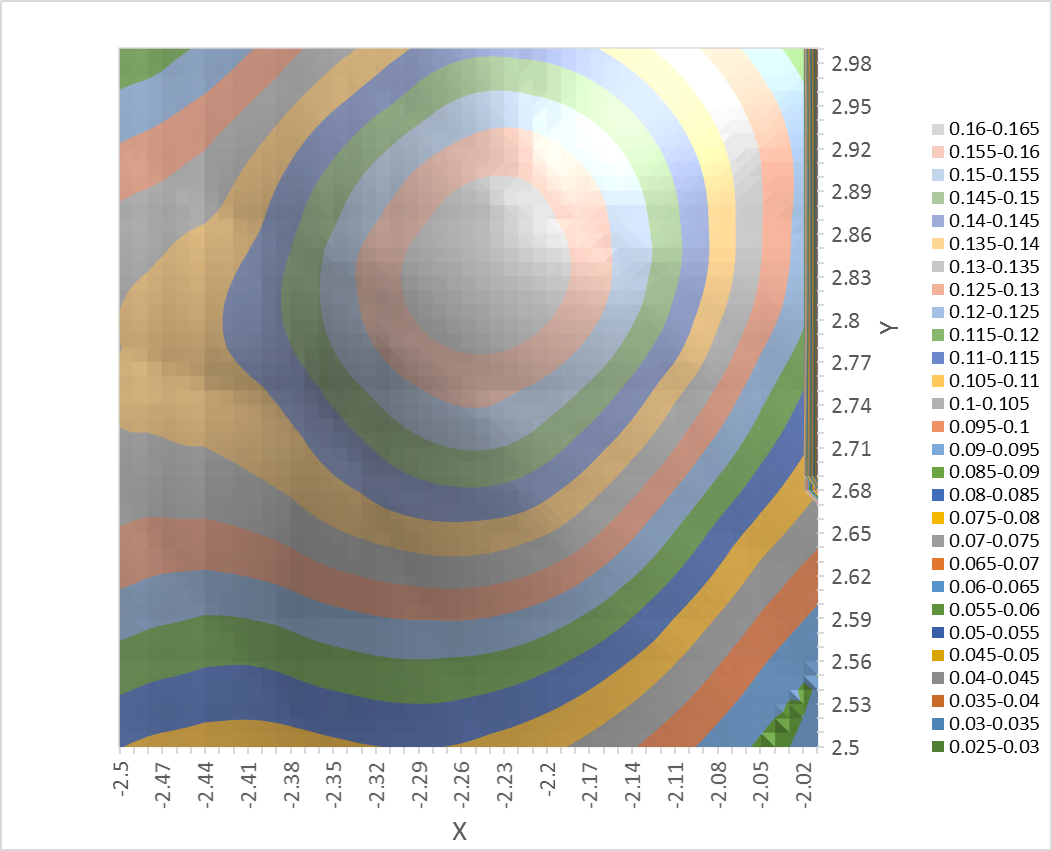
\includegraphics[width=9cm,keepaspectratio]{images/landscape_0_5.png}
	}
\end{subfigure}
	\caption[Fitness landscape peaks.]{High-precision sweep over peaks of scan110's fitness landscape, using different tolerances of sub sampling (left: 0.1, centre: 0.2, right: 0.5)}
	\label{fig:landscape_peaks}
\end{figure}

We hypothesise that this effect may be due to a coincidence in the data, such that a slight rotation and placement of the scan-points within a solid wall (surrounded by map points) would allow a higher fitness to occur. This could be detected by identifying continuous loops of points in a map, and penalising the placement of points within these 'solids' (accounting for some possible sensor error).


\subsection{Robustness to map topology}
\label{subsec:robustness_to_map_topology}
The issue does bring to light another significant assumption of our algorithm: the existence of a smooth global optima. This assumption allows consecutive small random mutations to 'crawl' an individual towards the global optima, thereby refining the pose. The same assumption also allows ICP to have an extremely high success rate, depending on the presence of a hypothetical pose which has a local maxima that is the map's global maxima. 

As demonstrated in our landscapes in \autoref{sec:fitness_landscape}, this does not appear to be the case for our test scans and maps. However, if exploring a repeated environment where features occur with slight variations (for example offices with desks, cabinets, walls), both the ICP-based algorithm and grid-pattern algorithm may converge to an incorrect maxima; depending on the density of the initial grid and the location of individuals within the local topology of the maxima. The inability to create fully new individuals through large mutations or crossovers would prevent either algorithm from searching unexplored areas.

The applicability of GA's to the problem of indoor localisation can then be subdivided into two cases, following intuition by \citet{Mitchell1998-td}; who considers the appropriateness of GAs to specific problems in relation to conventional 'weak' methods (which do not use domain-specific knowledge in their search procedure). \citeauthor{Mitchell1998-td} details that GA's are most applicable in non-smooth, non-unimodal search spaces; these would exist in the context of indoor localisation as feature-dense reference maps. However, if the search space isn't feature dense but does contain multiple peaks, it could be explored using the grid-based elitist GA, or the more efficient ICP-based algorithm in \autoref{subsec:icp_benchmark}. If available computational performance or memory are restricted, utilising the algorithms put forward by \citet{Robertson2002-ou} or \citet{Lenac2007-xm} would most likely 


When locating in smooth environments, the designed grid-based system provides a more efficient form of GA-based pose retrieval than our benchmark, but was demonstrated to be extremely inefficient compared to a basic global-ICP algorithm. However, as the environment becomes feature-dense (increasing the number of peaks in the fitness landscape) or large, these methods will require more memory and computational power (owing to the grid-initialisation), whereas the algorithms put forward by \citet{Robertson2002-ou} or \citet{Lenac2007-xm} may find a pose given a smaller memory usage but a larger computational time. 

As summarised by \citet{Mitchell1998-td}, the applicability of GA's depends greatly on the implementation's details, such as parameter settings and success criterion; the performance of the GA's may vary considerably, as demonstrated by the exhaustive parameter optimisations performed throughout this project. Whilst we have investigated the application of elitist selection and population priming to the problem of indoor localisation, it is important to note that the benefits provided by these design decisions do not benefit all possible cases.

\section{Further work}
As discussed in \autoref{subsec:robustness_to_map_topology}, variations in map topologies can cause some algorithms to solve the indoor localisation problem more efficiently than others. Defining a metric for a map which could determine which algorithm to utilise may be of value in applications; this could be related to the feature density, map size, similarity in repeated map features or other unexplored characteristics of maps. 

Further to this, the definition of a thorough and complete set of test scans and reference maps (which could be categorised in accordance with the aforementioned metric) could allow for a better understanding of the relative performance of algorithms, as the current research generally fails to use sufficiently varied test cases to provide a robust evaluation and comparison of algorithms.

\clearpage
\bibliographystyle{unsrt}
\bibliography{references}

\end{document}
